% !TeX encoding = UTF-8
% !TeX program = pdflatex
% !TeX spellcheck = en_US

\documentclass[LaM,binding=0.6cm,oneside]{sapthesis}

%\documentclass[oneside]{book}

% \usepackage{showframe}

\usepackage{indentfirst}
\usepackage{float}
\usepackage{graphicx}
\usepackage{caption}
\usepackage{subcaption}
\usepackage{setspace}
\usepackage{todonotes}
\usepackage{rotating}
\usepackage[utf8]{inputenc}
\usepackage{microtype}
\usepackage[english]{babel}
\usepackage[nottoc,numbib]{tocbibind}
\usepackage[hidelinks]{hyperref}
\usepackage{listings}
\usepackage{xcolor}
\usepackage{adjustbox}
\hypersetup{pdftitle={Analysis and Classification of 12-channel ECG signal using Edge Computing},pdfauthor={Hafiz Muhammad Hassan}}

% Commands for the titlepage
\title{Analysis and Classification of 12-channel ECG signal using Edge Computing}
\author{Hafiz Muhammad Hassan}
\IDnumber{1873829}
\course[override]{Corso di Laurea Magistrale in Data Science}
\courseorganizer{Facoltà di Ingegneria Dell'Informazione, Informatica e Statistica}
\AcademicYear{2021/2022}

\copyyear{2022}
\advisor{Prof. Ioannis Chatzigiannakis}

\authoremail{hassan.1873829@studenti.uniroma1.it}

\examdate{15 July 2022}
\examiner{Prof. Cuomo Francesca (Presidente)} 
\examiner{Prof. Anagnostopoulos Aristidis} 
\examiner{Prof. Brutti Pierpaolo}  
\examiner{Prof. Chatzigiannakis Ioannis}  
\examiner{Prof. Crespi Mattia} 
\examiner{Prof. Di Lorenzo Paolo}  
\examiner{Prof. Navigli Roberto} 




\begin{document}



\frontmatter

\maketitle
% \dedication{Dedicated to God, my family and my love one}





% \makeatletter
% \renewcommand{\SAP@AbstractLabel}{Abstract}
% \makeatother

\begin{acknowledgments}
\setstretch{1.125}
\parskip=12pt

I want to convey my gratitude to professor Ioannis Chatzigiannakis, my supervisor, for guiding me through thesis project with endeavour and commitment. It was a pleasant and educational journey to work under his leadership. I also extend this acknowledgement to Daniel and Lorella, my colleagues in this thesis, since they made spectacular contributions to this project.

I want to express my gratitude to my girlfriend Hasna, who supported me while developing this thesis with love and patience.

I also want to thank all faculty of data science program because they provided me with that knowledge that made me complete this thesis project. And last but not least, I would also like to thank family and friend for their support and contributions while studying in a foreign country.



\end{acknowledgments}

\tableofcontents

\mainmatter

\setstretch{1.125}
\parskip=5pt

\chapter{Introduction} \label{chap1}

The Fourth Industrial Revolution is fostering the emergence of new scenarios in which vast volumes of data are shared among independent and potentially disparate organizations. Often used on a cross-border basis to improve shared services in several sectors, such as finance and health care. Despite its benefits, technological advancements are introducing new security and privacy concerns associated with the use of these data, which include factors such as collection, analysis, usage, storage, and sharing. Indeed, in the case of personal information, incorrect usage, unsafe storage, data leakage, or misuse can all compromise a person's privacy. As a result, when personal data is subject to federated computation, the availability and proper use of privacy-preserving and fairness-aware mechanisms are presented as a key element to be addressed to increase people's trust and thus achieving the sustainable and ethical realization of these scenarios.

Digital Health Products (DHP) in the eHealth sector, in particular, present unique options to provide efficient, effective, cross-border high-quality healthcare services ~\cite{world2017global}. Today, cutting-edge AI-based medical data analysis has promise for early detection, faster diagnosis, better decision-making, and more successful treatment, according to ~\cite{arnold2017doctor}. The use of AI-based DHP in healthcare operations, services, and applications has created a significant and pressing need to combine highly private medical data gathered from a variety of sources. It also includes millions of parameters that must be learned from sufficiently big, curated datasets to reach clinical-grade accuracy while remaining safe, fair, and equitable, as well as generalizing well to previously unseen ~\cite{wang2019deep}.

Federated learning (FL) is an architecture that aims to solve the problem of data governance and privacy by collectively training algorithms without transferring data. It was originally designed for a variety of domains, including mobile and edge device use cases, but it has recently acquired popularity in healthcare applications \cite{intro}. FL allows for collaborative insights, such as in the form of a consensus model, without transferring patient data outside of the institutions' firewalls. Instead, each participating institution's ML process takes place locally, with only model weights being shared. Models trained by FL can achieve performance levels comparable to those trained on centrally hosted data sets and superior to models that only see isolated single-institutional data, according to recent studies \cite{intro}.

% Review for introduction: 
% - https://www.nature.com/articles/s41746-020-00323-1


\section{Document's outline} \label{doc_struct}

The present thesis document is organized into six chapters. 

The first chapter (\ref{chap1}) introduces the reasons behind the need for a machine learning solution to classify the 12-leads, encouraging the introduction of Federated Learning in the architecture. The second chapter (\ref{chap2}) describes the essential background to understand the cardiological basics. It contains the human heart nature and all the concepts associated with ECG monitoring, including the most common arrhythmia types.

The third chapter (\ref{chap3}) focuses on the state-of-the-art regarding the research topic. It contains information for both ECG classification and Federated Learning. In the fourth chapter (\ref{chap4}), the analytical methodologies and tools are introduced and explained in detail. 

The fifth chapter (\ref{chap5}) it is exposed the results of analyzing the proposed data under both the Centralized and Federated Learning environment. Finally, the last chapter (\ref{chap6}) is dedicated to the overall conclusions achieved by the research and to possible future developments.

\chapter{Cardiological fundamentals} \label{chap2}

\cite{ecg1} "An electrocardiogram (ECG) is a measure of how the electrical activity of the heart changes over time, as action potentials within each myocyte propagate throughout the heart as a whole during each cardiac cycle. In other words, the ECG is the recording of the cumulative signals produced by populations of cells eliciting changes in their membrane potentials at a given point in time. The ECG provides specific waveforms of electrical differences when the atria and ventricles depolarize and repolarize."

\section{The human heart nature} \label{heart_nature}

For the purposes of an ECG, the human body can be thought of as a large volume conductor. It is made up of tissues and a conductive media in which the heart is suspended. The heart contracts during the cardiac cycle in response to coordinated action potentials traveling through the chambers of the heart. One section of the heart tissue is depolarized, while another is at rest or polarized, as is usual. 

The intensity of the voltages observed is determined by the electrodes' orientation in relation to the dipole ends. The signal amplitudes are proportional to the mass of tissue used to create the dipole at any particular time. Electrodes are typically placed on the skin's surface to detect the voltages of these electrical fields, giving rise to the ECG \cite{ecg1}.

\begin{figure}[H]
\centering
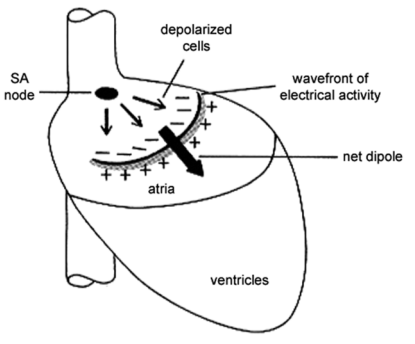
\includegraphics[scale=0.7]{img/heart_nature.PNG}
\caption{After conduction begins at the sinoatrial node, cells in the atria begin to depolarize. This creates an electrical wavefront that moves down toward the ventricles, with polarized cells at the front. The separation of charge results in a dipole across the heart (the large black arrow shows its direction) \cite{ecg1}.}
\label{fig:heart_nat}
\end{figure}


\section{ECG's history} \label{ecg_history}

The discovery of intrinsic electrical activity within the heart dates all the way back to the 1840s. Carlo Matteucci, an Italian physicist, was the first to discover that each heartbeat is accompanied by an electrical current in 1842. Emil DuBois-Reymond, a German scientist, published the first action potential associated with muscular contraction not long after. In 1856, Rudolph von Koelliker and Heinrich Miller used a galvanometer to record the first cardiac action potential. Following that, Augustus D. Waller recorded the first human ECG after Gabriel Lippmann invented the capillary electrometer in the early 1870s. That first device is shown in Figure \ref{fig:Kapillarelektrometer}.

\begin{figure}[H]
\centering
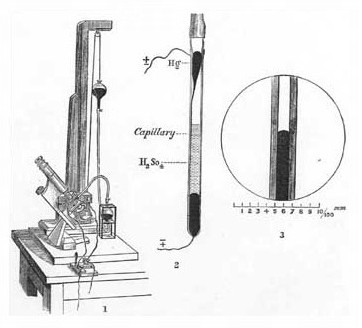
\includegraphics[scale=0.5]{img/Kapillarelektrometer.jpg}
\caption{Lippmann electrometer}
\label{fig:Kapillarelektrometer}
\end{figure}

Willem Einthoven's creation of the string galvanometer in 1901 was a key milestone in cardiac electrocardiography. The next year, he published the first ECG using his string galvanometer. Einthoven's string galvanometer consisted of a huge electromagnet with a thin silver-coated string stretched across it; electric currents passing through the thread caused the string to move from side to side in the electromagnet's magnetic field.


Einthoven made yet another significant addition to cardiac electrophysiology in 1912, when he discovered a mathematical link between the direction and size of the deflections recorded by the three limb leads. Einthoven's triangle is the name for this hypothesis. Before Frank Wilson described unipolar leads and the precordial lead configuration, the typical three-limb leads were used for three decades. The traditional Einthoven limb leads, as well as the precordial and unipolar limb leads based on Wilson's work, make up the 12-lead ECG layout now in use.


This instrument was initially manufactured in 1905 by the Cambridge Scientific Instrument Company in London. Electrical impulses were sent from a hospital over a mile away to Einthoven's laboratory via a telephone cable. Bedside machines, on the other hand, were not available until the 1920s. The Sanborn Company produced a smaller version of the unit in 1935 that weighed only about 25 pounds.

\begin{figure}[H]
\centering
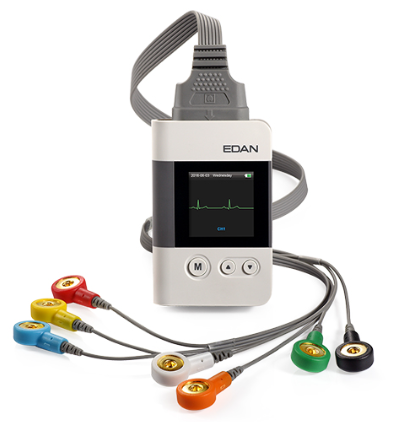
\includegraphics[scale=0.7]{img/holter_edan_ecg.PNG}
\caption{Holter-Edan ECG device}
\label{fig:holter_monitor}
\end{figure}

With Norman Jeff Holter's invention of the Holter monitor in 1949, the use of ECG in a nonclinical context became viable. The first iteration of this device was a 75-pound backpack that could record the ECG continually and send the signals via radio. The size of subsequent iterations of such devices has been drastically decreased, and the signal is now recorded digitally. Miniaturized devices now allow patients to be monitored for longer periods of time (typically 24 hours) to aid in the diagnosis of any rhythm or ischemic heart disease concerns. One of the latest versions of the ECG is the one appearing in Figure \ref{fig:holter_monitor}.

\section{The ECG Waveform} \label{ecg_waveform}

Signals of voltage versus time are created during the recording of an ECG, which are generally shown in millivolts (mV) vs seconds. Figure \ref{fig:ECG_waveform} depicts a typical Lead II ECG waveform. The negative electrode was placed on the right wrist and the positive electrode on the left ankle for this Lead II ECG recording. As a result, a series of peaks and waves can be seen, each of which corresponds to ventricular or atrial depolarization and repolarization, with each segment of the signal indicating a separate event in the cardiac cycle.

\begin{figure}[H]
\centering
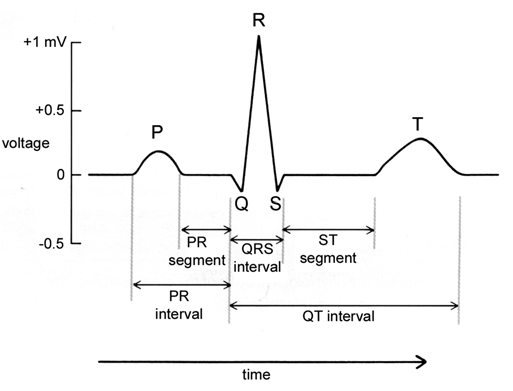
\includegraphics[scale=0.7]{img/ECG_waveform.PNG}
\caption{A typical ECG waveform for one cardiac cycle, measured from the Lead II position \cite{ecg1}.}
\label{fig:ECG_waveform}
\end{figure}
 
Three principal waveforms are recorded by the ECG (\ref{fig:ECG_waveform}):

\begin{itemize}
    \item The P-wave
    \item QRS complex
    \item T-wave.
\end{itemize}

The P-wave is created by depolarisation of the atria, the QRS by depolarisation of the ventricles, and the T-wave by repolarisation of the ventricles. In most people, these waveforms occur in a repeating rhythm called sinus rhythm, so called because it originates in the sinus node. In some people, a fourth waveform (not shown in the previous image) called a U-wave can be seen. This is usually seen at slower heart rates. The significance of the U-wave remains uncertain. Some authors think that it represents the late stages of ventricular repolarisation, while others describe it as a post-repolarisation phenomenon. U-wave abnormalities have been described in various disease states including ischaemic heart disease \cite{ecg2}.
 
 The depolarization of the sinoatrial node, which is positioned within the right atrium, starts the typical cardiac cycle. A conventional ECG will not detect this early firing because the node does not have enough cells to provide a measurable electrical potential. The right and left ventricles continue to depolarize after the P wave, resulting in the recordable QRS complex, which lasts about 100 milliseconds. The Q-wave is the initial negative deflection (if present), the R-wave is the largest positive deflection, and the S-wave is the smallest positive deflection \cite{ecg3}.
 
 
 The T-wave is usually the last potential in a cardiac cycle, followed by the P-wave of the next cycle, and so on. The ECG signal returns to baseline near the conclusion of ventricular contraction, and the ventricles repolarize after contraction. Atrial contractions have stopped and the atria are repolarizing at the same time as the QRS complex. Because the effects of this widespread atrial repolarization are obscured by the much larger volume of tissue engaged in ventricular depolarization, it is not generally detectable in an ECG \cite{ecg1}. 
 
 
\section{The 12-leads ECG} \label{12_lead_ecg}

An ECG lead is a recording of the heart's electrical activity as seen from one side. As a result, when we take a 12-lead ECG, we're recording cardiac electrical activity from 12 different angles \cite{ecg3}. Assume you're visiting a historic structure and taking images of it. If you snap 12 photos from different angles around the structure, each one will depict a distinct element, such as the front, sides, and back. They work together to provide a three-dimensional record of the structure's shape and appearance. In a similar way, a 12-lead ECG creates a three-dimensional depiction of the heart's electrical activity.

\begin{figure}[H]
\centering
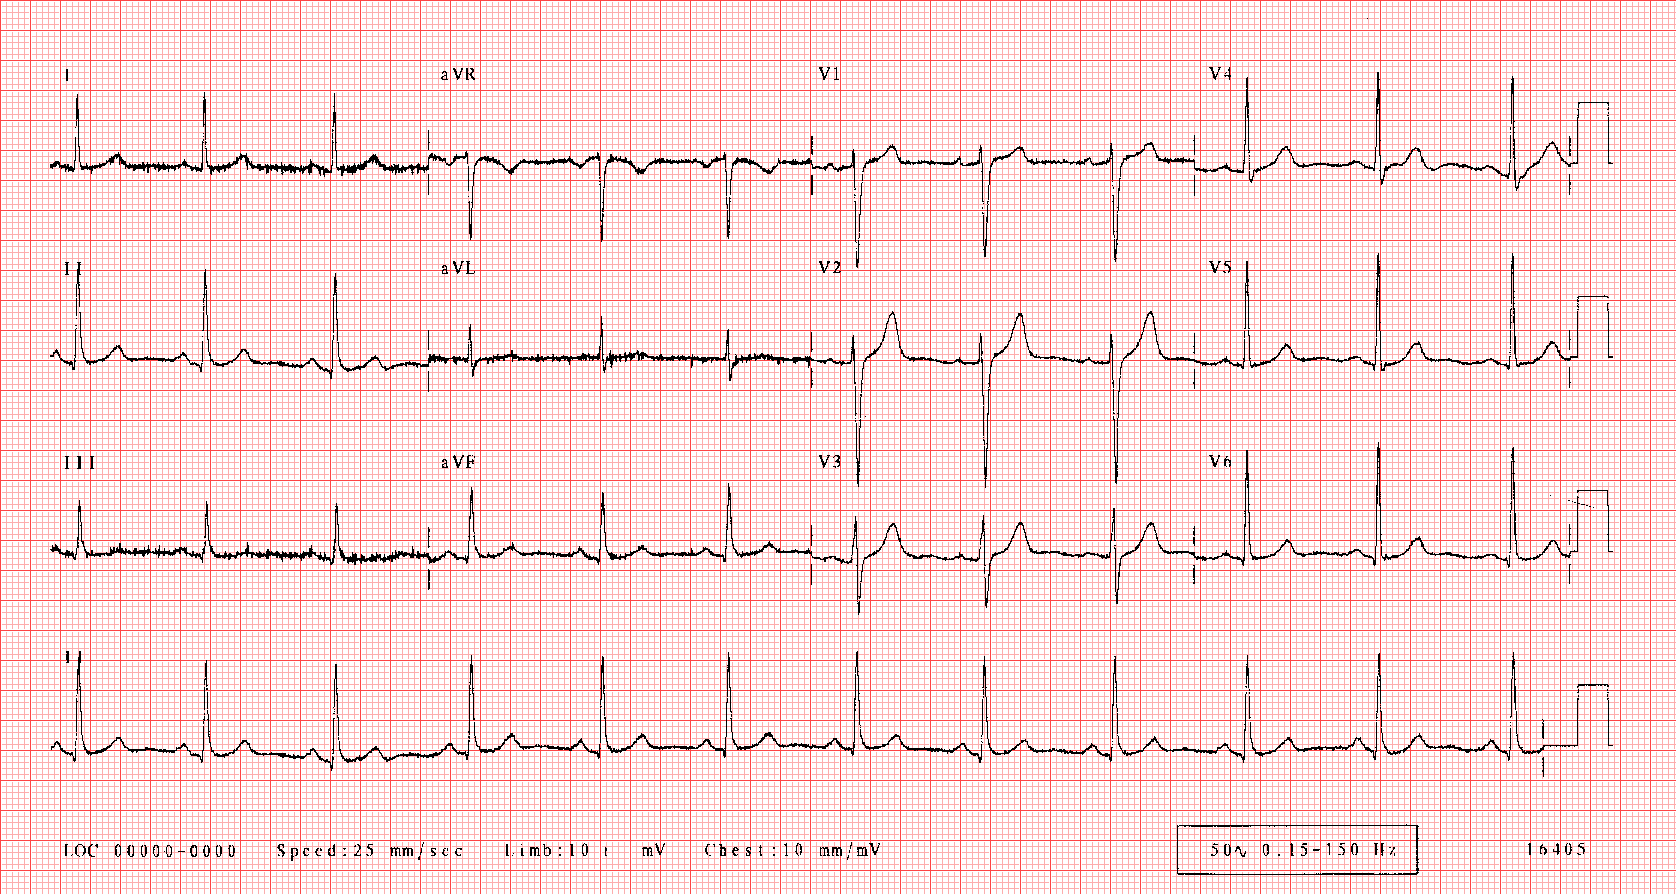
\includegraphics[scale=0.24]{img/normal_ecg.png}
\caption{12-leads normal ECG}
\label{fig:normal_ecg}
\end{figure}

Multiple images of the heart's electrical activity can be recorded depending on the type of machine utilized and the number of electrodes inserted. The usage of 12-lead ECG devices is common among health-care professionals. Twelve separate electrical images of the heart are measured and recorded via a 12-lead ECG (Figure \ref{fig:normal_ecg}). In other words, it records the electrical activity of the heart as observed from 12 various angles. For example, Lead II monitors electrical activity as observed from the heart's inferior (diaphragmatic) surface. This lead is frequently used to measure heart rate \cite{basic_arryth}.

\section{Arrhythmias Types} \label{arrhythmias_types}

Analyzing arrhythmias is a difficult undertaking since every person on the planet has a unique ECG that differs from everyone else's, and one person's ECG can change dramatically from one second to the next. Memorizing some of the most common ECG patterns and attempting to recognize them in the future is insufficient. Pattern identification is a popular yet unintentional way of approaching arrhythmias via ECG analysis (\cite{arryth_types}). Often the Arrhythmias are divided into two global categories:

\begin{enumerate}
    \item \textbf{Rhythmic}: Determined as a sequence of uneven beats
    \item \textbf{Morphological}: Made of abnormal single beat
\end{enumerate}

The work presented in the current thesis is focused on first type of classification. Those arrhythmias have a categorization provided by SNOMED CT. The latter is the world's most complete and precise terminology package, with widespread acceptance around the world. It provides a common language for clinical IT systems, making data exchange between them easier, safer, and more accurate. It covers everything from processes and symptoms to clinical measurements, diagnosis, and drugs, and it's all in one place.

For the Physionet 2020 challenge were only considered around 27 arrhythmias, which are the most frequently found regarding the ECG analysis. Nevertheless, along the following paragraphs there is a deep explanation of all the possible arrhythmias. To see the complete list of categories it is possible to read the GitHub cited in \cite{github_arrhythmias}.

Arrhythmias are often divided into groups based on where the rhythm is initiated by the pacemaker. The following are the most prevalent sites, and consequently the primary arrhythmia categories:

\begin{enumerate}
    \item Sinus
    \item Atrial
    \item Junctional
    \item Ventricular
    \item AV Blocks
\end{enumerate}

\subsection{Sinus}

It is necessary to comprehend the 'benchmark' rhythm, or hemodynamically perfect rhythm, which is referred to as \textbf{Normal Sinus Rhythm} and sometimes abbreviated to \textbf{NSR}, in order to assess cardiac rhythms (Figure \ref{fig:nsr}). The following features must be present in order for a rhythm to be classified as Normal Sinus Rhythm:

\begin{table}[H]
\begin{center}
\begin{tabular}{||c || c||}
 \hline
\textbf{Characteristic} & \textbf{Status} \\ [0.4ex] 
 \hline\hline
Rhythm & Regular \\
\hline
Rate & 60-100/minute \\
\hline
p waves & Present, upright, symmetrical, one before every QRS \\
\hline
pri & .12-.20 seconds \\
\hline
QRS & .06-.10 seconds \\
\hline\hline
\end{tabular}
\end{center}
\caption{Characteristics of Normal Sinus Rhythm}
\label{table:nsr_characteristics}
\end{table}


\begin{figure}[H]
\centering
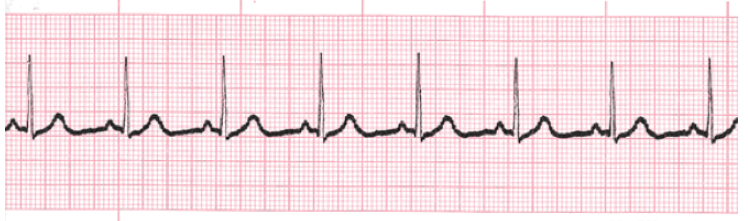
\includegraphics[scale=0.65]{img/NSR.png}
\caption{Normal Sinus Rhythm (\cite{arryth_types})}
\label{fig:nsr}
\end{figure}
 
\textbf{Sinus Bradycardia (SB)}: When a patient's heart rate falls below 60 beats per minute, they are said to be bradycardic. Slow heart rates can be seen in fit and active people who are usually asymptomatic. When a patient's heart rate falls below 60 beats per minute, critical care nurses must be ready to assess for decreasing cardiac output right away.

\begin{table}[H]
\begin{center}
\begin{tabular}{||c || c||}
 \hline
\textbf{Characteristic} & \textbf{Status} \\ [0.4ex] 
 \hline
 Rhythm & Regular \\
\hline\hline
Rate & < 60/minute \\
\hline
p waves & Present, upright, symmetrical, one before every QRS \\
\hline
pri & .12-.20 seconds \\
\hline
QRS & .06-.10 seconds \\
\hline\hline
\end{tabular}
\end{center}
\caption{Characteristics of Sinus Bradycardia}
\label{table:sb_characteristics}
\end{table}


 \begin{figure}[H]
\centering
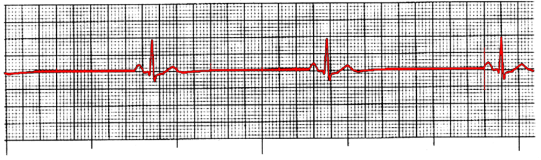
\includegraphics[scale=0.85]{img/SB.png}
\caption{Sinus Bradycardia (\cite{arryth_types})}
\label{fig:sb}
\end{figure}

\textbf{Sinus Tachycardia (STach)}: When a patient's heart rate exceeds 100 beats per minute, they are labeled tachycardic, though most people don't notice symptoms until their heart rate exceeds 150 beats per minute. At this point, a critical care nurse should look for signs and symptoms of decreased cardiac output (such as hypotension or a loss of consciousness).

\begin{table}[H]
\begin{center}
\begin{tabular}{||c || c||}
 \hline
\textbf{Characteristic} & \textbf{Status} \\ [0.4ex] 
 \hline\hline
 Rhythm & Regular \\
\hline
Rate & >100/minute \\
\hline
p waves & Present, upright, symmetrical, one before every QRS \\
\hline
pri & .12-.20 seconds \\
\hline
QRS & .06-.10 seconds \\
\hline\hline
\end{tabular}
\end{center}
\caption{Characteristics of Sinus Tachycardia}
\label{table:STach_characteristics}
\end{table}


 \begin{figure}[H]
\centering
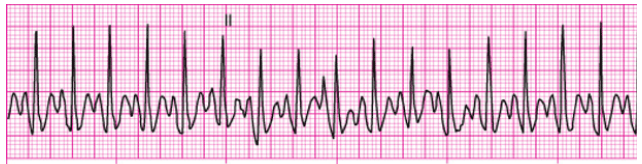
\includegraphics[scale=0.8]{img/STach.png}
\caption{Sinus Tachycardia (\cite{arryth_types})}
\label{fig:STach}
\end{figure}

\textbf{Sinus Arrhythmia (SA)}: This arrhythmia is typically benign and do not require any sort of treatment. It is seen in children and also in mechanically ventilated patients.

\begin{table}[H]
\begin{center}
\begin{tabular}{||c || c||}
 \hline
\textbf{Characteristic} & \textbf{Status} \\ [0.4ex] 
 \hline\hline
 Rhythm & Regular \\
\hline
Rate & 60-100/minute \\
\hline
p waves & Present, upright, symmetrical, one before every QRS \\
\hline
pri & .12-.20 seconds \\
\hline
QRS & .06-.10 seconds \\
\hline\hline
\end{tabular}
\end{center}
\caption{Characteristics of Sinus Arrhythmia}
\label{table:SA_characteristics}
\end{table}


 \begin{figure}[H]
\centering
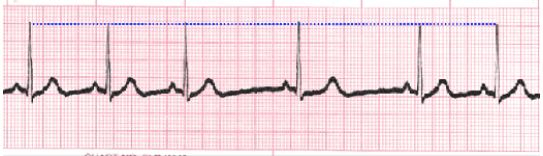
\includegraphics[scale=0.9]{img/SA.png}
\caption{Sinus Arrhythmia (\cite{arryth_types})}
\label{fig:SA}
\end{figure}

\textbf{Wandering Atrial Pacemaker (WAP)}: It can be a normal aberration associated to Ischemia. There is no treatment required.

\begin{table}[H]
\begin{center}
\begin{tabular}{||c || c||}
 \hline
\textbf{Characteristic} & \textbf{Status} \\ [0.4ex] 
 \hline\hline
 Rhythm & Regular \\
\hline
Rate & 60-100/minute \\
\hline
p waves & P waves vary in shape and size \\
\hline
pri & .12-.20 seconds \\
\hline
QRS & .06-.10 seconds \\
\hline\hline
\end{tabular}
\end{center}
\caption{Characteristics of Wandering Atrial Pacemaker}
\label{table:WAP_characteristics}
\end{table}


 \begin{figure}[H]
\centering
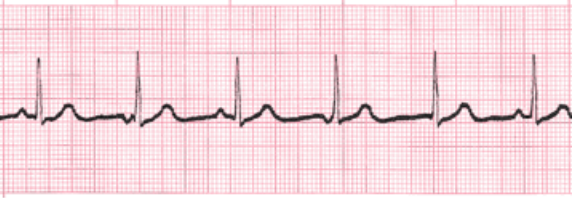
\includegraphics[scale=0.9]{img/WAP.png}
\caption{Wandering Atrial Pacemaker (\cite{arryth_types})}
\label{fig:WAP}
\end{figure}

\subsection{Atrial}

The rhythms that originate in the atrial will be examined in the following section. Premature atrial contractions, atrial flutter, atrial fibrillation, and supraventricular tachycardia are examples of these arrhythmias. The key characteristics of cardiac rhythms will be outlined, as well as nursing consequences and useful advice to help critical care nurses correctly interpret atrial arrhythmias.

\textbf{Premature Atrial Contractions (PAC)}: it can be a normal aberration,
Ischemia,  or a signal of atrial irritability. It can lead to more serious atrial rhythms.

\begin{table}[H]
\begin{center}
\begin{tabular}{||c || c||}
 \hline
\textbf{Characteristic} & \textbf{Status} \\ [0.4ex] 
 \hline\hline
 Rhythm & Early beat (PAC) causes rhythm to be irregular \\
\hline
Rate & Underlying rhythm usually 60-100/minute\\
\hline
p waves & P waves have different configuration than underlying rhythm \\
\hline
pri & .12-.20 seconds in underlying rhythm \\
\hline
QRS & .06-.10 seconds in underlying rhythm \\
\hline\hline
\end{tabular}
\end{center}
\caption{Characteristics of Premature Atrial Contractions}
\label{table:PAC_characteristics}
\end{table}

 \begin{figure}[H]
\centering
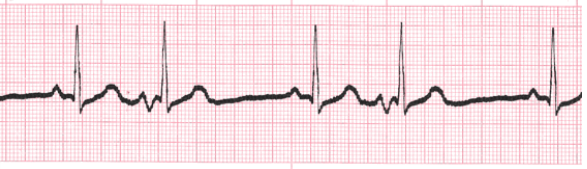
\includegraphics[scale=0.9]{img/PAC.png}
\caption{Premature Atrial Contractions (\cite{arryth_types})}
\label{fig:PAC}
\end{figure}

\textbf{Atrial Flutter (AFL)}: It is caused by electrolyte imbalance, Hypertension, Ischaemic heart disease, Congenital heart disease, Rheumatic valve disease. Also after a cardiac surgery.

\begin{table}[H]
\begin{center}
\begin{tabular}{||c || c||}
 \hline
\textbf{Characteristic} & \textbf{Status} \\ [0.4ex] 
 \hline\hline
 Rhythm & Regular or irregular \\
\hline
Rate & 60-100/minute (ventricular rate) 250-400 (atrial rate)\\
\hline
p waves & No p waves present. Flutter waves (F waves) or ‘sawtooth’ waves \\
\hline
pri & No pri since no p waves \\
\hline
QRS & .06-.10 seconds \\
\hline\hline
\end{tabular}
\end{center}
\caption{Characteristics of Atrial Flutter}
\label{table:AFL_characteristics}
\end{table}

 \begin{figure}[H]
\centering
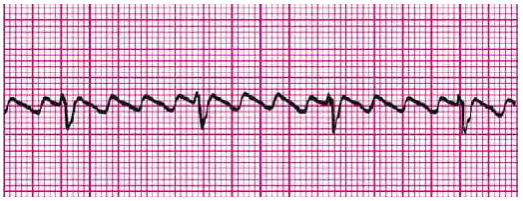
\includegraphics[scale=0.9]{img/AFL.png}
\caption{Atrial Flutter (\cite{arryth_types})}
\label{fig:AFL}
\end{figure}

\textbf{Atrial Fibrillation (AF)}: It is caused by Electrolyte imbalance, Hypertension, Ischaemic heart disease, Congenital heart disease, Rheumatic valve disease. Also following a cardiac surgery.

\begin{table}[H]
\begin{center}
\begin{tabular}{||c || c||}
 \hline
\textbf{Characteristic} & \textbf{Status} \\ [0.4ex] 
 \hline\hline
 Rhythm & Irregular \\
\hline
Rate & 60-100/minute (ventricular rate) >400/minute (atrial rate)\\
\hline
p waves & No p waves. Fibrillatory waves (f waves) \\
\hline
pri & No No pri since no p waves \\
\hline
QRS & .06-.10 seconds \\
\hline\hline
\end{tabular}
\end{center}
\caption{Characteristics of Atrial Fibrillation}
\label{table:AF_characteristics}
\end{table}

 \begin{figure}[H]
\centering
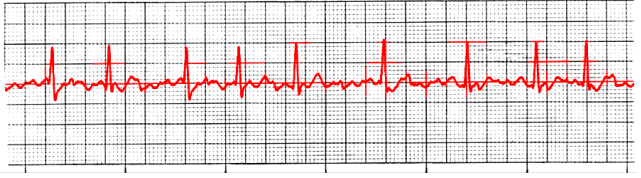
\includegraphics[scale=0.8]{img/AF.png}
\caption{Atrial Fibrillation (\cite{arryth_types})}
\label{fig:AF}
\end{figure}

\textbf{Supraventricular Tachycardia (SVT)}: It is caused by Congenital, heart disease, Emotional stress, Physical stress or exertion, Illegal drugs (i.e. Cocaine or ecstasy), Alcohol, Caffeine.

\begin{table}[H]
\begin{center}
\begin{tabular}{||c || c||}
 \hline
\textbf{Characteristic} & \textbf{Status} \\ [0.4ex] 
 \hline\hline
 Rhythm & Regular \\
\hline
Rate & 150-250/minute (atrial rate)\\
\hline
p waves & P waves may not be seen at higher rates \\
\hline
pri & .12-.20 seconds (if seen) \\
\hline
QRS & .06-.10 seconds \\
\hline\hline
\end{tabular}
\end{center}
\caption{Characteristics of Supraventricular Tachycardia}
\label{table:SVT_characteristics}
\end{table}

 \begin{figure}[H]
\centering
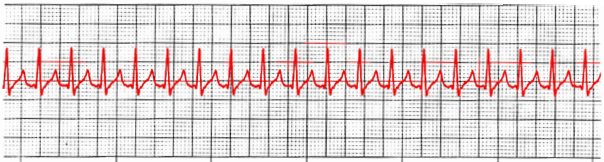
\includegraphics[scale=0.9]{img/SVT.png}
\caption{Supraventricular Tachycardia (\cite{arryth_types})}
\label{fig:SVT}
\end{figure}

\subsection{Junctional}

Junctional rhythms are temporary and non-lethal rhythms that originate in the AV node or junctional region. Inverted p waves are a typical feature of all junctional rhythms. Premature junctional contractions, junctional rhythm, and paroxysmal junctional tachycardia are among the rhythms covered in this section (\cite{arryth_types}).


\textbf{Premature Junctional Contraction (JPC)}: It is caused by Medication toxicity (i.e. digoxin), Ischemia. There is not treatment required.
Continue to observe for increasing number of JPCs since this indicates
increasing AV node irritability.


\begin{table}[H]
\begin{center}
\begin{tabular}{||c || c||}
 \hline
\textbf{Characteristic} & \textbf{Status} \\ [0.4ex] 
 \hline\hline
 Rhythm & Early beat (PJC) causes the rhythm to be irregular \\
\hline
Rate & 60-100/minute (underlying rhythm)\\
\hline
p waves & P waves inverted or not seen in JPC \\
\hline
pri & Not applicable \\
\hline
QRS & .06-.10 seconds (in underlying rhythm) \\
\hline\hline
\end{tabular}
\end{center}
\caption{Characteristics of Premature Junctional Contraction}
\label{table:JPC_characteristics}
\end{table}

 \begin{figure}[H]
\centering
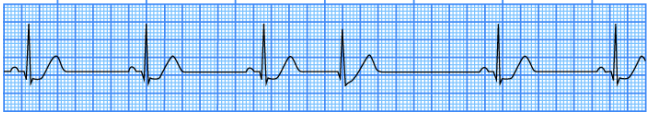
\includegraphics[scale=0.8]{img/JPC.png}
\caption{Premature Junctional Contraction (\cite{arryth_types})}
\label{fig:JPC}
\end{figure}


\textbf{Junctional Rhythm (AVJR)}: It is caused by Medication toxicity (i.e. digoxin) or ischemia. It is necessary to treat causes.


\begin{table}[H]
\begin{center}
\begin{tabular}{||c || c||}
 \hline
\textbf{Characteristic} & \textbf{Status} \\ [0.4ex] 
 \hline\hline
 Rhythm & Regular \\
\hline
Rate & <60/minute \\
\hline
p waves & P waves inverted or absent \\
\hline
pri & .12-.20 seconds \\
\hline
QRS & .06-.10 seconds \\
\hline\hline
\end{tabular}
\end{center}
\caption{Characteristics of Junctional Rhythm}
\label{table:AVJR_characteristics}
\end{table}

 \begin{figure}[H]
\centering
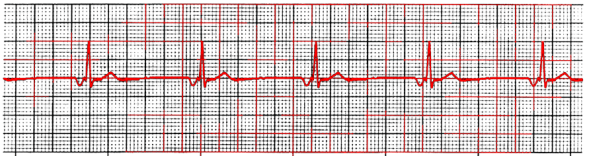
\includegraphics[scale=0.9]{img/AVJR.png}
\caption{Junctional Rhythm (\cite{arryth_types})}
\label{fig:AVJR}
\end{figure}


\textbf{Accelerated Junctional Rhythm (AJR)}: It is caused by Medication toxicity (i.e. digoxin) or ischemia. It is necessary to treat causes.

\begin{table}[H]
\begin{center}
\begin{tabular}{||c || c||}
 \hline
\textbf{Characteristic} & \textbf{Status} \\ [0.4ex] 
 \hline\hline
 Rhythm & Regular \\
\hline
Rate & 60-100/minute \\
\hline
p waves & P waves inverted or absent \\
\hline
pri & Not applicable \\
\hline
QRS & .06-.10 seconds \\
\hline\hline
\end{tabular}
\end{center}
\caption{Characteristics of Accelerated Junctional Rhythm}
\label{table:AJR_characteristics}
\end{table}

 \begin{figure}[H]
\centering
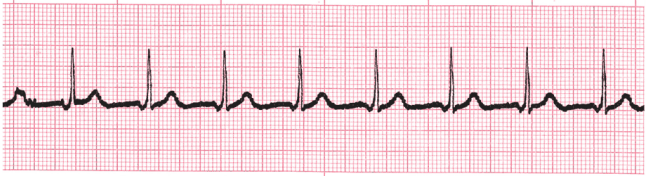
\includegraphics[scale=0.8]{img/AJR.png}
\caption{Accelerated Junctional Rhythm (\cite{arryth_types})}
\label{fig:AJR}
\end{figure}

\textbf{Paroxysmal Junctional Tachycardia (JT)}: It is caused by ischemia. Its treatment is the same than SVT.

\begin{table}[H]
\begin{center}
\begin{tabular}{||c || c||}
 \hline
\textbf{Characteristic} & \textbf{Status} \\ [0.4ex] 
 \hline\hline
 Rhythm & Regular \\
\hline
Rate & 150-250/minute \\
\hline
p waves & P waves inverted or absent (if seen) \\
\hline
pri & Not applicable \\
\hline
QRS & .06-.10 seconds \\
\hline\hline
\end{tabular}
\end{center}
\caption{Characteristics of Paroxysmal Junctional Tachycardia}
\label{table:JT_characteristics}
\end{table}

 \begin{figure}[H]
\centering
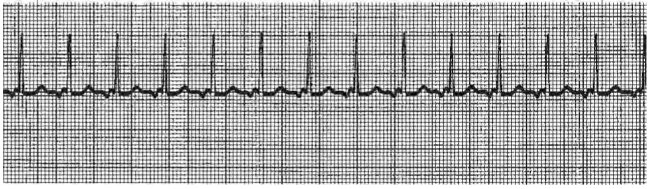
\includegraphics[scale=0.8]{img/JT.png}
\caption{Paroxysmal Junctional Tachycardia (\cite{arryth_types})}
\label{fig:JT}
\end{figure}


\subsection{Ventricular}

Premature ventricular contractions, ventricular tachycardia, and ventricular fibrillation are examples of ventricular rhythms that can be induced by irritability, as well as those that result from the failure of higher-level pacemakers. Irritability patients have significantly various treatment options and consequences.

\textbf{Premature Ventricular Contractions (PVC)}: It is caused by Ventricular irritability (i.e.hypoxemia, acid-base imbalance, medications, electrolyte imbalance).

\begin{table}[H]
\begin{center}
\begin{tabular}{||c || c||}
 \hline
\textbf{Characteristic} & \textbf{Status} \\ [0.4ex] 
 \hline\hline
 Rhythm & Early beat (PVC) causes the rhythm to be irregular \\
\hline
Rate & 60-100/minute (underlying rhythm) \\
\hline
p waves & None (in PVC) \\
\hline
pri & None (in PVC) \\
\hline
QRS & > .12 seconds (wide and bizzare) \\
\hline\hline
\end{tabular}
\end{center}
\caption{Characteristics of Premature Ventricular Contractions}
\label{table:PVC_characteristics}
\end{table}

 \begin{figure}[H]
\centering
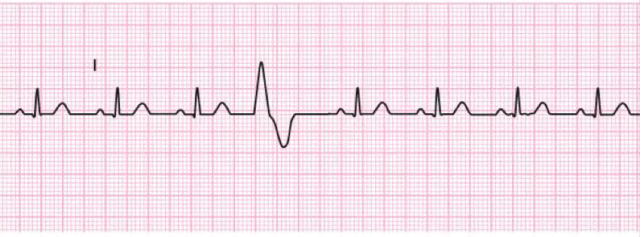
\includegraphics[scale=0.8]{img/PVC.png}
\caption{Premature Ventricular Contractions (\cite{arryth_types})}
\label{fig:PVC}
\end{figure}

\textbf{Ventricular Tachycardia (VTach)}: It is caused by Ventricular irritability (i.e.hypoxemia, acid-base imbalance, medications, electrolyte
imbalance).

\begin{table}[H]
\begin{center}
\begin{tabular}{||c || c||}
 \hline
\textbf{Characteristic} & \textbf{Status} \\ [0.4ex] 
 \hline\hline
 Rhythm & Regular \\
\hline
Rate & 150-250/min \\
\hline
p waves & None  \\
\hline
pri & None  \\
\hline
QRS & > .12 seconds (wide and bizzare) \\
\hline\hline
\end{tabular}
\end{center}
\caption{Characteristics of Premature Ventricular Contractions}
\label{table:VTach_characteristics}
\end{table}

 \begin{figure}[H]
\centering
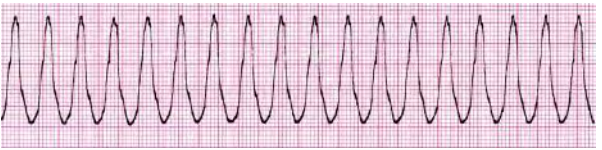
\includegraphics[scale=0.8]{img/VTach.png}
\caption{Premature Ventricular Contractions (\cite{arryth_types})}
\label{fig:VTach}
\end{figure}

\textbf{Ventricular Fibrillation (VF)}: It is caused by Ventricular irritability (i.e.hypoxemia, acid-base imbalance, medications, electrolyte
imbalance).

\begin{table}[H]
\begin{center}
\begin{tabular}{||c || c||}
 \hline
\textbf{Characteristic} & \textbf{Status} \\ [0.4ex] 
 \hline\hline
 Rhythm & Irregular and chaotic \\
\hline
Rate & Cannot calculate \\
\hline
p waves & None  \\
\hline
pri & None  \\
\hline
QRS & None \\
\hline\hline
\end{tabular}
\end{center}
\caption{Characteristics of Ventricular Fibrillation}
\label{table:VF_characteristics}
\end{table}

 \begin{figure}[H]
\centering
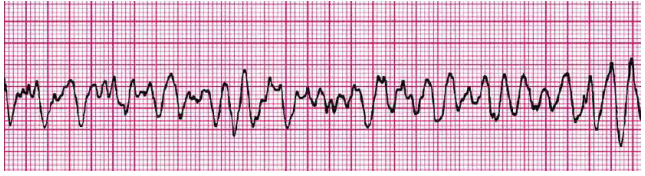
\includegraphics[scale=0.8]{img/VF.png}
\caption{Ventricular Fibrillation (\cite{arryth_types})}
\label{fig:VF}
\end{figure}

\textbf{Idioventricular Rhythm (IR)}: It is caused by Ischemia, reperfusion post thrombolytics.

\begin{table}[H]
\begin{center}
\begin{tabular}{||c || c||}
 \hline
\textbf{Characteristic} & \textbf{Status} \\ [0.4ex] 
 \hline\hline
 Rhythm & Regular \\
\hline
Rate & <40/minute \\
\hline
p waves & No p waves  \\
\hline
pri & No pri  \\
\hline
QRS & > .12 seconds (wide and bizarre) \\
\hline\hline
\end{tabular}
\end{center}
\caption{Characteristics of Idioventricular Rhythm}
\label{table:IR_characteristics}
\end{table}

 \begin{figure}[H]
\centering
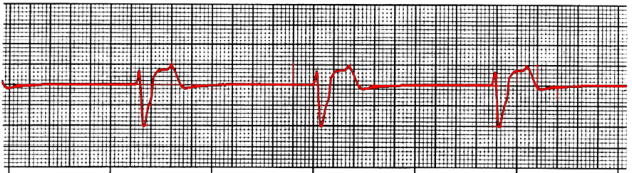
\includegraphics[scale=0.8]{img/IR.png}
\caption{Idioventricular Rhythm}
\label{fig:IR}
\end{figure}


\subsection{AV Blocks}

Electrical conduction failure via the myocardium is characterized by atrioventricular (AV) blockages. Because AV blockages are linked to severe risk worsening or haemodynamic impairment, the critical care nurse must recognize and treat them as soon as possible. 1st degree heart block, 2nd degree heart block (Mobitz type 1 or Wenkebach), and 3rd degree heart block are all types of AV block (complete heart block).  (\cite{arryth_types})

\textbf{First Degree AV Block (IAVB)}: It is caused by AV nodal disease, Enhanced vagal tone (i.e. athletes), Myocarditis, Following Myocardial Infarction, Electrolyte disturbances, Medications (i.e. Calcium channel blockers, Beta blockers).

\begin{table}[H]
\begin{center}
\begin{tabular}{||c || c||}
 \hline
\textbf{Characteristic} & \textbf{Status} \\ [0.4ex] 
 \hline\hline
 Rhythm & Regular \\
\hline
Rate & 60-100/minute \\
\hline
p waves & P waves normal  \\
\hline
pri & >.20 seconds     \\
\hline
QRS & .06-.10 seconds \\
\hline\hline
\end{tabular}
\end{center}
\caption{Characteristics of First Degree AV Block}
\label{table:IAVB_characteristics}
\end{table}

 \begin{figure}[H]
\centering
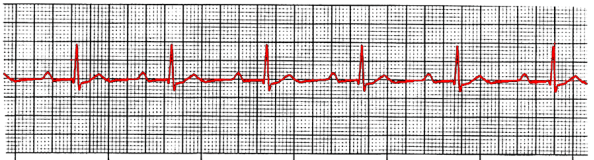
\includegraphics[scale=0.8]{img/IAVB.png}
\caption{First Degree AV Block (\cite{arryth_types})}
\label{fig:IAVB}
\end{figure}


\textbf{Second Degree Type I (IIAVB)}: It is caused by Ischemia. Usually benign, with no treatment required. If patient becomes haemodynamically compromised interventions for bradycardia should be considered.


\begin{table}[H]
\begin{center}
\begin{tabular}{||c || c||}
 \hline
\textbf{Characteristic} & \textbf{Status} \\ [0.4ex] 
 \hline\hline
 Rhythm & Regular or slightly irregular \\
\hline
Rate & 60-100/minute \\
\hline
p waves & P waves normal  \\
\hline
pri & Progressively gets longer until a beat is dropped     \\
\hline
QRS & .06-.10 seconds \\
\hline\hline
\end{tabular}
\end{center}
\caption{Characteristics of Second Degree Type I}
\label{table:IIAVB_characteristics}
\end{table}

 \begin{figure}[H]
\centering
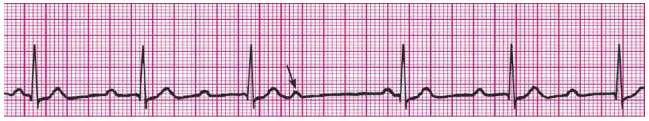
\includegraphics[scale=0.8]{img/IIAVB.png}
\caption{Second Degree Type I (\cite{arryth_types})}
\label{fig:IIAVB}
\end{figure}




\chapter{Related work} \label{chap3}

\section{Bibliographical research methodology} \label{3biblio_research}

To define the state-of-the-art for ECG classification and Edge Computing. I performed a reduced Systematic Review. The latter is defined as \cite{systematic_review} a 'process of critically evaluating, summarizing, and seeking to reconcile the evidence.' In other words, it is a complete evaluation of literature that differs from a traditional review in that it is undertaken in a methodical (or systematic) manner, following a pre-specified process to avoid bias, with the goal of synthesizing the information gathered. 

Then the first step to perform the systematic review (SR or bibliographical research) was to decide the reference and citation databases to use. In the table \ref{table:dbs_sr} are written the academic search engines used to retrieve the related documents.

\begin{table}[H]
\begin{center}
% \resizebox{\textwidth}{!}{
\begin{tabular}{||p{0.2\linewidth} || p{0.55\linewidth} | p{0.15\linewidth}||}
 \hline
\textbf{Search Engine} & \textbf{Definition} & \textbf{Link} \\ [0.4ex] 
 \hline\hline
Google Scholar & A free web search engine that indexes the full text or metadata of scholarly literature from a variety of publishers and fields. & \href{https://scholar.google.com/}{Link to GS} \\
\hline
PubMed.gov & Contains almost 34 million citations from MEDLINE, life science journals, and online books for biomedical literature. & \href{https://pubmed.ncbi.nlm.nih.gov/}{Link to PM} \\
\hline
IEEEXplore & A research database that allows users to access journal articles, conference proceedings, technical standards, etc. in computer science, electrical engineering, and electronics. & \href{https://ieeexplore.ieee.org/Xplore/home.jsp}{Link to IE} \\
\hline
Scopus & Has a huge collection of Physical Sciences and Engineering papers, from foundational science to novel and unique research, and spanning many disciplines both theoretical and applied. & \href{https://www.sciencedirect.com/}{Link to SCs} \\
\hline
Web Of Science & It is the most reliable publisher-independent worldwide citation database in the world. & \href{https://clarivate.com/webofsciencegroup/solutions/web-of-science/}{Link to WoS} \\
\hline
Papers with code & Their goal is to provide a free and open library that includes Machine Learning articles, code, datasets, methodologies, and evaluation tables. & \href{https://paperswithcode.com/}{Link to PwC} \\
\hline\hline
\end{tabular}
% }
\end{center}
\caption{Databases (search engines) used to find documents}
\label{table:dbs_sr}
\end{table}

Each one of the search engines showed in the previous table work based on a "query" which will contain the information of the topic desired. Besides, to get better results, it is recommended to use multiple queries that may enrich the matter in research. Those queries are listed below, grouped by the specific topic to be found about:

\begin{enumerate}
    \item \textbf{Edge Computing Generalities}: To retrieve the conceptual definition and approximations of Edge Computing I used the following queries:
    \begin{itemize}
        \item Edge Computing arrhythmia
        \item Edge Computing ECG
        \item Edge Computing healthcare arrhythmia
        \item Edge Computing healthcare iot
        \item Edge Computing IoT ecg
        \item Edge Computing healthcare low power mobile
        \item Edge Computing PhysioNet
        \item Edge Computing TensorFlow Lite
    \end{itemize}
    \item \textbf{Options for ECG classification}: To get the different methods used along the history in the ECG classification theme I employed the next queries:
    \begin{itemize}
        \item Machine Learning ECG arrhythmia
        \item Deep Learning ECG arrhythmia
        \item Machine Learning IoT ECG arrhythmia
        \item Deep Learning IoT ECG arrhythmia
    \end{itemize}
    
    As I am going to use Federated Learning technique for edge computing, I employed these techniques. 
    
    \item \textbf{Non-IID Methods}: To evaluate the different methods to deal with Non Independent Nor Identical distributed (Non-IID) data, I search over the following queries:
    \begin{itemize}
        \item Federated learning non iid
        \item Federated learning independent identically distributed
    \end{itemize}
    \item \textbf{Imbalanced data}: To check the techniques used by other authors regarding the class (labels, response variable) imbalanced, I used the next queries:
    \begin{itemize}
        \item Imbalanced data ecg
        \item Imbalanced data federated learning
    \end{itemize}
    \item \textbf{Metrics}: To gather the most used metrics in both ECG and Federated Learning ECG classifications I employed the following queries:
    \begin{itemize}
        \item Federated learning metrics
        \item ECG classification metric
    \end{itemize}
    \item \textbf{Federated learning types}: To understand the possible architectures of Federated Learning I was based on the next queries:
    \begin{itemize}
        \item Federated learning architecture
        \item Types federated learning
    \end{itemize}
    \item \textbf{Arrhythmia types}: To know the different arrhythmia classifications, I employed the following query:
    \begin{itemize}
        \item Cardiac Arrhythmia types
    \end{itemize}
\end{enumerate}


2480 articles were found using the queries mentioned previously. It is important to mention that for each one of those queries, I downloaded the results retrieved in BibTex and CSV formats, depending on the search engine used. With the files saved it was possible to retrieve some generalities from the documents. As an example, in figure \ref{fig:timeline_papers} it is depicted the number of papers found in each search database divided by publication year.

 \begin{figure}[H]
\centering
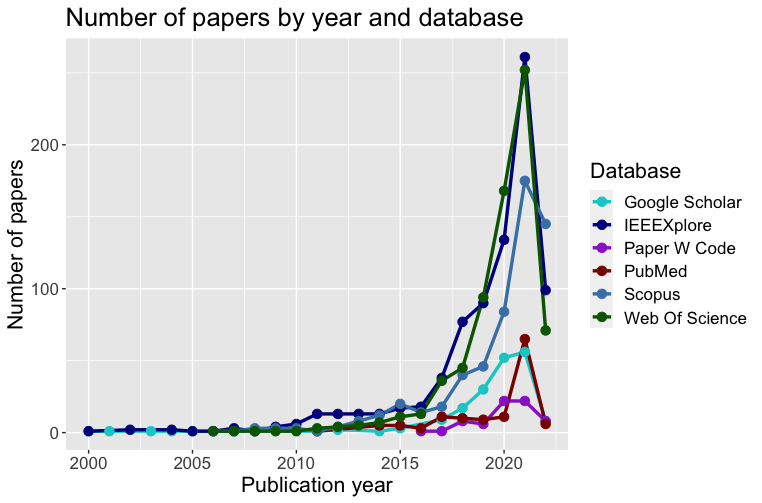
\includegraphics[scale=0.54]{img/timeline_papers.png}
\caption{PRISMA flow for gathering documents}
\label{fig:timeline_papers}
\end{figure}


From the previous graph we can see that most of the papers were published after 2017-2018. At the same time we can see that most of them got published in peak on 2021. ECG classification is a topics that has been worked back in the 2000s. Moreover, the search engine that produced the highest number of resources was IEEEXPlore. 


\section{ECG classification} \label{3state_art_ECG}

After reading the aforementioned documents which was already screened, I gather some relevant highlights regarding the classification of ECG signals. Along the following paragraphs I summarize the most important findings at each topic.

\subsection{Techniques to handle imbalanced data}

In general, imbalanced data describes datasets in which the target class has an unequal distribution of observations. For example, when one class label has a large number of observations while the other has a small number.The authors who have dealt with this topic followed different paths to tackle this issue. Authors from \cite{imbalance_data1} introduced a \textit{Balanced Accuracy (BACC)} and the \textit{Matthew’s Correlation Coefficient (MCC)} to correct the fact that the classes don't share a similar distribution. In the article \cite{imbalance_data2} it was introduced the \textit{Generative Adversarial Network (GAN)} which deals with imbalanced data by generating and using additional fake data for detection purpose. In addition, \cite{imbalance_data3} used the \textit{Synthetic Minority Oversampling Technique (SMOTE)}, which is an oversampling technique. 

Other approaches also include the so-called \textit{Ratio Loss} (\cite{imbalance_data4}) where the global node estimates the composition data each round. When detecting an imbalanced composition continuously, the system acknowledges the class imbalance and load the Ratio Loss. One final possibility is the \textit{Recall of data} in which one randomly augment the lower class and in each training epoch change the selected individuals. Then, there are enough possibilities tried in the literature, each of of them with their pros and cons that can be verified further.


\subsection{Methods for ECG classification} \label{methods_ECG_class}

Along the literature I could find that a huge amount of diverse techniques have been applied when classifying ECG' arrhythmias. As an example \cite{ecg_methods1}, \cite{ecg_methods2}, and \cite{ecg_methods3} focused their efforts on Using Deep Neural Networks (Artificial Neural Networks and Multi-layer Perceptron) to get a model that predicts the abnormality given the ECG signal. In comparison, the author of \cite{ecg_methods4} combined in his paper the use of Naïve Bayes, Adaboost, Random Forest and Support Vector Machines to get the best classifier for his paper. Finally, \cite{ecg_methods5}, \cite{ecg_methods6} and \cite{ecg_methods7} employed in their research some Convolutional Neural Network approaches. Among them the highlighted Squeezenet, Attention mechanism and Resnet as the champion methods to deal with the ECG detection.

 \begin{figure}[H]
\centering
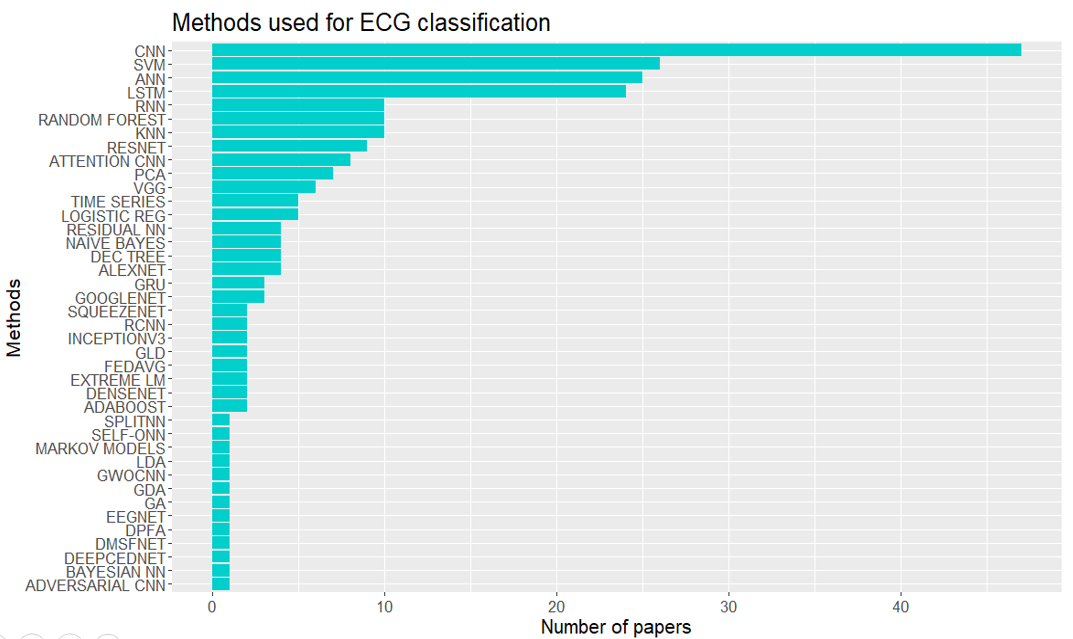
\includegraphics[scale=0.48]{img/classif_methods.PNG}
\caption{Most used classification methods for ECG}
\label{fig:classif_methods}
\end{figure}

As depicted in figure \ref{fig:classif_methods}, the most used technique is the Convolutional Neural Network (CNN). That one includes also some self-made Deep Neural Networks (DNN). On the second place we find Support Vector Machines (SVM) and Artificial Neural Networks (ANN). An very close to them most of the author also used Long-Short Term Memory (LSTM) algorithms. On the opposite, a few papers contributed with techniques like GWOCNN, DFPA, DEEPCETNET, etc, which are also CNN but that have specific alterations adapted to by the papers' authors.

\subsection{Metrics for ECG classification}\label{chap3metrics}

With respect to ECG arrhythmia classification, there are plenty of measurements employed in the literature. In figure \ref{fig:metrics_ECG} I show the most relevant metrics used in this aim, gathered from the available articles and papers shown in chapter \ref{3biblio_research}. 

 \begin{figure}[H]
\centering
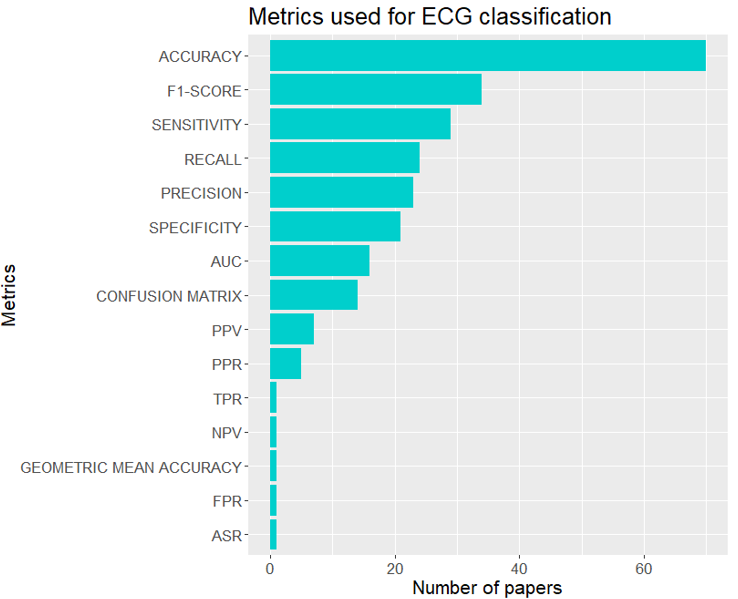
\includegraphics[scale=0.48]{img/metrics_ECG.PNG}
\caption{Most used metrics for ECG}
\label{fig:metrics_ECG}
\end{figure}

From the previous chart it is evident that the most used measure is the \textbf{Accuracy}. In the second place, the \textit{F1-Score} is often used. It is important to clarify that the latter is preferred when dealing with unbalanced data, since it take into account both \textit{Recall} and \textit{Precision} for its calculation. Some papers that consider the 4 mentioned measures at the same time can be found in \cite{metrics_ecg1}, 
\cite{metrics_ecg2} and \cite{metrics_ecg3}.


\subsection{Edge computing using Federated Learning} \label{fedrated_learning_as_edge computing}

To understand how we can we use Fedrated learning as Edge computing. This paper \cite{fedrated_learning_as_edge_computing} is published on 2021 which states that Federated Learning is a machine learning scheme in which a shared prediction model can be collaboratively learned by a number of distributed nodes using their locally stored data. It can provide better data privacy because training data are not transmitted to a central server. Federated learning is well suited for edge computing applications and can leverage the the computation power of edge servers and the data collected on widely dispersed edge devices.

Edge federated learning solves the data island problem by fully exploring the huge potential of the data on terminal devices like mobiles or small iot devices without infringing on user’s privacy, and it greatly improves the efficiency of model learning in edge computing systems usually edge server.  Therefore, it can be widely used in many scenarios where privacy protection and resource utilization are critical. It can apply to healthcare system, vehicular network and intelligent recommendation. 


\subsection{Methods to handle NON-IID data} \label{non_iid_handling}

Along the literature, the researches performed have been focused on tackling the Non Independent Nor Identical distributed (Non-IID) problem that make the models in FL under-perform. In the following part I present a summary of the most relevant techniques used to deal with the mentioned issue.

\textbf{Over/under-sampling}: This is one of the most common techniques used to balance the data. It consist of randomly creating (or removing) data to equate distributions. The simplest way to do it is called Random Oversampling (ROS). The latter is the process of randomly picking and replacing instances from the minority class in the training dataset. There are other techniques like SMOTE \cite{metrics_ecg1}. SMOTE is a data augmentation algorithm that creates synthetic data points depending on the original data points. The technique can be thought of as a more advanced variant of oversampling or as a specific data augmentation process. SMOTE has the advantage of not creating duplicate data points, but rather synthetic data points that are somewhat different from the original data points \cite{imbalance_data3}.

\begin{figure}[H]
\centering
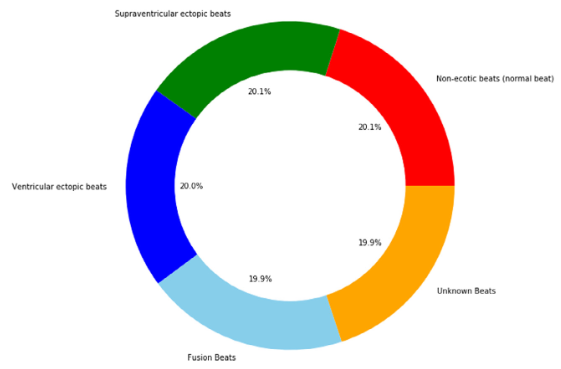
\includegraphics[scale=0.6]{img/metrics_ecg1_ROS.PNG}
\caption{The distribution of the up-sampled (re-balanced) dataset. \cite{metrics_ecg1}}
\label{fig:metrics_ecg1_ROS}
\end{figure}



\textbf{Data sharing strategy}: In the paper \cite{fl18} they showed that for neural networks trained with highly skewed non-IID data, where each client device trains just on a single class of data, the accuracy of federated learning drops by up to 55\%. They also showed that the weight divergence, which can be measured by the Earth mover's distance (EMD) between the distribution over classes on each device and the population distribution, can explain the loss in accuracy. As a solution, the proposal was to establish a limited sample of data that is globally shared across all edge devices to improve training on non-IID data. Their proposed data sharing is exposed in the following image:

\begin{figure}[H]
\centering
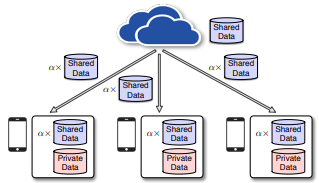
\includegraphics[scale=0.9]{img/fl18_datasharing.PNG}
\caption{ Illustration of the data-sharing strategy. \cite{fl18}}
\label{fig:fl18_datasharing}
\end{figure}





\textbf{Fedprox}: FedProx uses Federated Average Aggregation (FedAvg) to improve the local aim. It restricts the size of local updates directly. To limit the distance between the local model and the global model, it adds an additional L2 regularization term to the local objective function. This is a simple approach to keep the local updates under control so that the averaged model stays close to the global optima. To regulate the weight of the L2 regularization, a hyper-parameter is introduced \cite{fl19}.

\subsection{Metrics for Federated Learning}

Inside the FL framework the same metrics showed in \ref{chap3metrics} are often used. In the ECG case, metrics like Accuracy, F1-Score, Recall and Precision are usually employed to measure the overall capacity of the model to detect the diagnoses. I will be usually using the same metrics to evaluate the performance of the each node which can be acting as edge server(global node) or edge node(local node). 


\subsection{PhysioNet/Computing in Cardiology Challenge 2020}

\subsubsection{Introudction and Keypoints}

As I am going to use \cite{physionet_challenge_2020} PhysioNet/Computing in Cardiology Challenge 2020 dataset. It is often good to consider and finding out what papers has been published and what kind of architecture they were following. 

\cite{main_arythmia_detection}To encourage more multidisciplinary researches, PhysioNet in Cardiology Challenge 2020 (Challenge 2020) \cite{physionet_challenge_2020} provided high-quality 12-lead ECG data obtained from multiple centers with a large set of cardiac abnormalities. The aim of Challenge 2020 was to identify clinical diagnoses from 12-lead ECG recordings, providing an opportunity to employ various advanced methods to address clinically important questions that are either unsolved or not well-solved \cite{arythmia_detection_9}.

Later I did the specific analysis specifically considering the papers published during conference. 41 teams got selected during this challenge and others are simply discarded because the method did not work on the hidden set, the team failed to submit a preprint or a final article on time, or the team was absent during CinC conference. Looking at the 41 teams papers published in PhysioNet \cite{physionet_challenge_2020}. One can observe that some techniques are used by the majority of the teams. The results indicate that ECG classification is a complex process that includes multiple techniques. Among these techniques, signal processing, DNNs, convolutional neural networks (CNNs), end-to-end and multi-binary classifications are used by all of the top 10 teams. In addition, there are several important points 1) deep-learning methods were more popular than traditional methods in Challenge 2020; 2) all the teams that employed deep-learning methods used CNNs; and 3) none of the top-10 teams used hand-labeled features (except demographic features); they all adopted end-to-end models instead. 

To investigate the techniques applied by each team, I considered five aspects of the methods that formed a solution pipeline (see \ref{fig:meta_analysis_2020_teams}): data preprocessing, feature engineering, machine-learning models, training strategy, and applications to the real world. Table 2 presents these five aspects.


\begin{figure}[H]
\centering
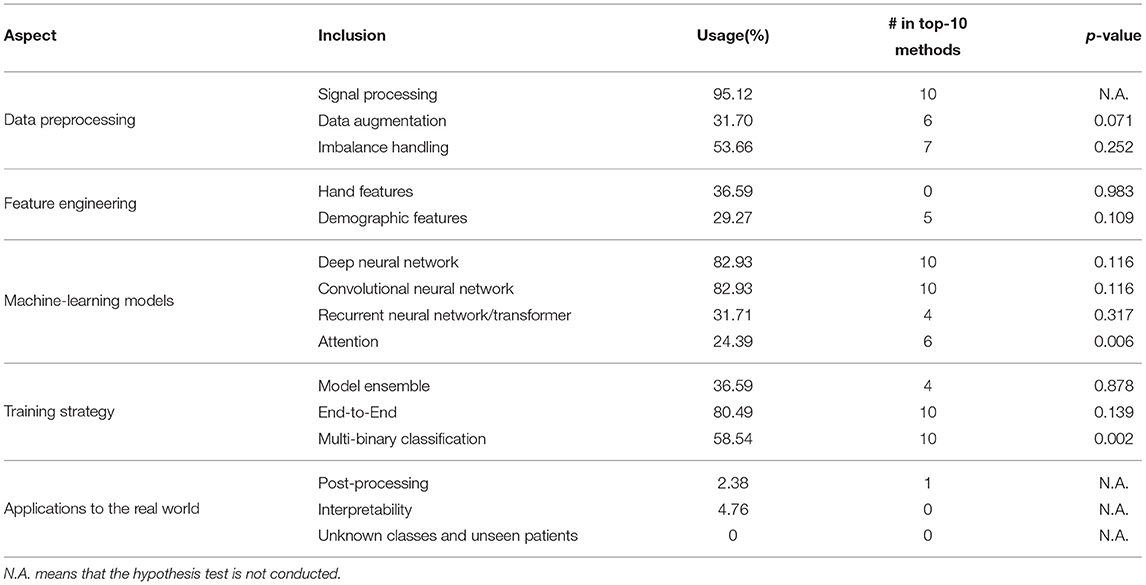
\includegraphics[scale=0.32]{img/meta_analysis_2020_teams.jpeg}
\caption{Details of employed techniques.}
\label{fig:meta_analysis_2020_teams}
\end{figure}


\cite{main_arythmia_detection} One can also notice that the three highest-ranking teams used the model ensemble \cite{first_team, second_team, third_team}, but only 14 out of 41 teams employed this strategy. It is also important to note that model ensemble only helps if used for single model rather than models that are structurally different. Most of team also used only age and sex as features rather other using demographic features or 12-lead ECG based features. The training data in Challenge 2020 suffer from heavy class imbalance (as shown in \ref{fig:label_ditro_alldata}) so most teams used  threshold optimization \cite{eighth_team, second_team, ninth_team} and weighted loss \cite{sixth_team, seventh_team} to handle imbalance class issue. In addition, over-sampling \cite{thirteen_team}, down-sampling \cite{sixteen_team}, and other methods have been employed in Challenge 2020.

\subsubsection{Practical Lessons:}

\begin{enumerate}
  \item Data augmentation should be employed and adapted to specific scenarios.
  \item Combining different features can improve performance.
  \item A hybrid design of different types of deep neural networks (DNNs) is better than using a single type.
   \item The use of end-to-end architectures should depend on the task being solved.
   \item Multiple models are better than one.
\end{enumerate}

\subsubsection{Finding open source algorithms from Published Papers}

To find open source code of the papers I have search them in Google and Github, I was able to find the source code of 9 papers that was accepted during the challenge including team 2, team 6 and team 20. I will be later using these source code for analysis try to incorporate some additional features that i have identified during centralized learning approach of Fedarated learning. 

It is important to note that \textbf{Pytorch} is most widely used framework by participants implementation of the Physionet Challenge 2020. [\ref{fig:framework_used_by_2020_teams}]. 'Not Mentioned' either represents that they didn't wrote in their paper what kind of implementation they are following or I am not able to find out their implementation of the paper on the internet. 

\begin{figure}[H]
\centering
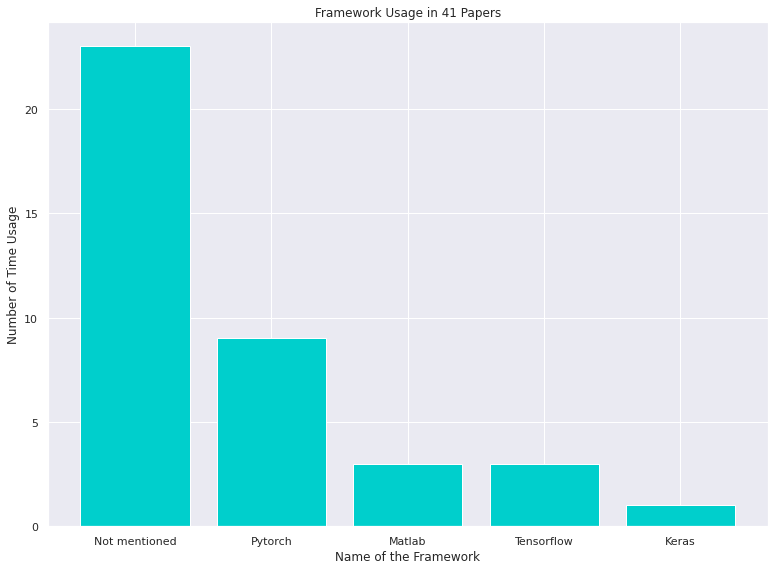
\includegraphics[scale=0.5]{img/framework_usage_in_papers.png}
\caption{Most used framework during Physionet Challenge 2020}
\label{fig:framework_used_by_2020_teams}
\end{figure}

I have also created an excel sheet which has combination of the meta analysis of 2020 challenge \cite{main_arythmia_detection} and all the open source code related to each team participated in the challenge. Which can be found here: https://bit.ly/3bgFtWs 



\chapter{Analytical techniques and tools} \label{chap4}

The parts that follow go over the most important analysis and approaches for studying, modelling, and predicting ECG arrhythmia diagnosis.

\section{Commonly used techniques and tools} \label{4commontools}

\subsection{Data Wrangling (DW)} \label{4dw}

Data wrangling is the act of cleaning and combining chaotic and difficult data sets for easy access and analysis. With the amount of data and data sources growing all the time, it's more vital than ever to arrange massive volumes of data for analysis \cite{datawrang}. To facilitate data consumption and organization, this method normally requires manually transforming and mapping data from one raw format to another.

The most relevant Data Wrangling objectives are \cite{datawrang}:

\begin{itemize}
    \item Collect data from a variety of sources to uncover "deeper intelligence."
    \item As soon as feasible, get reliable, actionable data into the hands of business analysts.
    \item Reduce the amount of time it takes to collect and organize jumbled data before it can be used.
    \item Allow data scientists and analysts to focus on data analysis instead of data manipulation.
    \item Encourage senior executives in a company to improve their decision-making skills.
\end{itemize}

\begin{figure}[H]
\centering
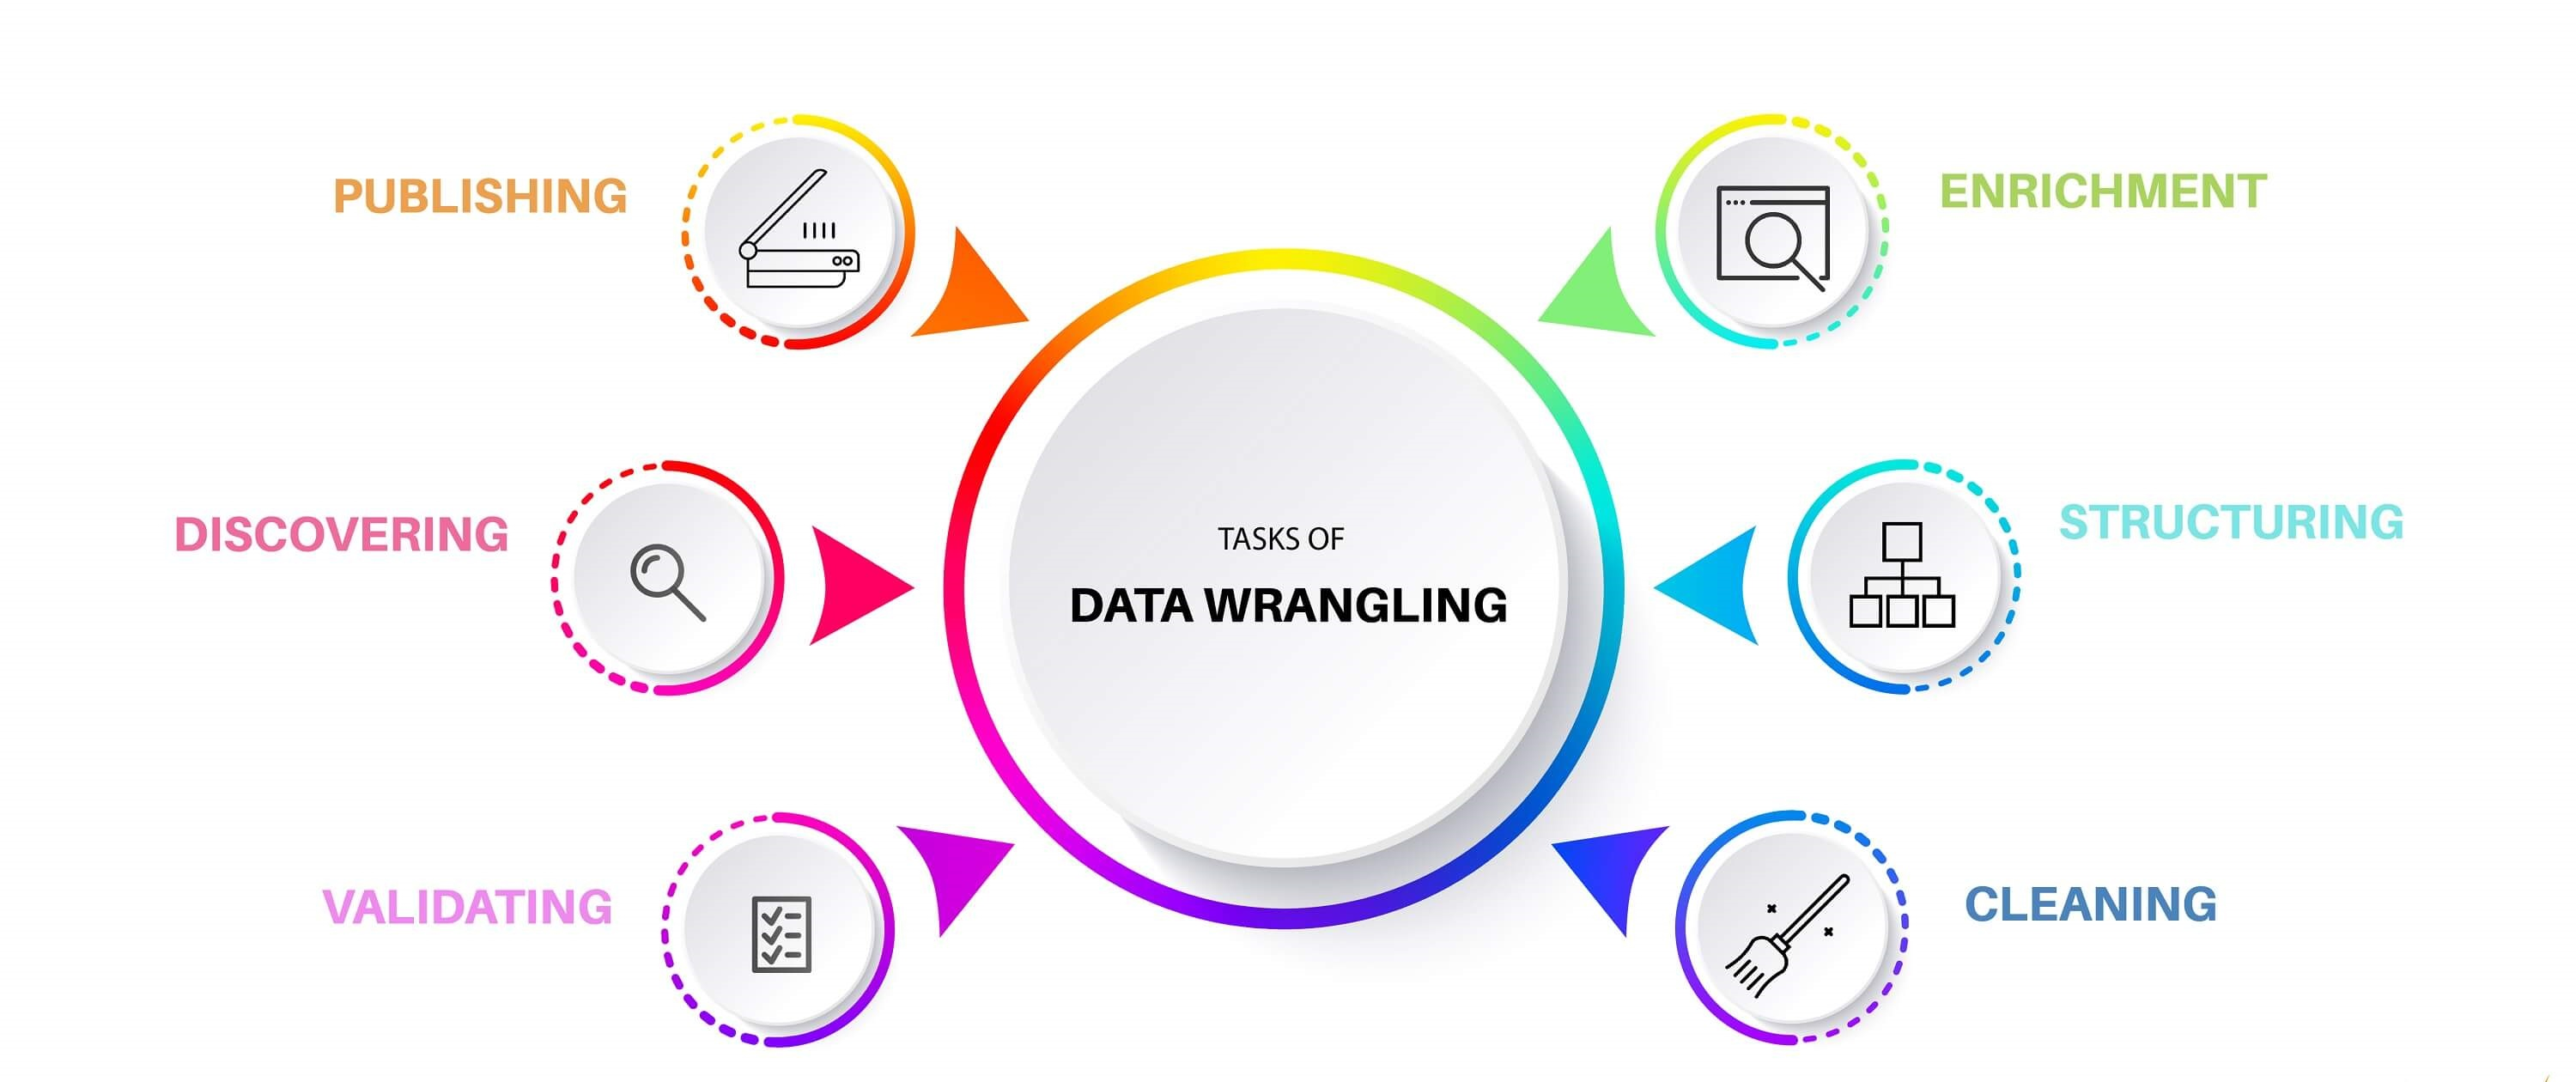
\includegraphics[scale=0.18]{img/DATA_WRANGLING.jpg}
\caption{Main steps in Data Wrangling}
\label{fig:dwprocess}
\end{figure}

The data wrangling approach typically consists of six iterative steps, as seen in Figure \ref{fig:dwprocess}, as mentioned by \cite{datawrang2}:

\begin{enumerate}
    \item \textbf{Publishing:} Data wranglers prepare data for downstream usage - whether by a specific user or program - and identify any special actions or logic that were employed to do so. 
    
    \item \textbf{Discovering:} Before delving into the data, it's important to first have a better knowledge of what's there since this will influence how you examine the data.

    \item \textbf{Validating:} These are recurrent programming sequences that verify data quality, consistency, and security. Validation can include things like ensuring that qualities that should be distributed regularly are distributed uniformly.
    
    \item \textbf{Enrichment:} "What more types of data can be obtained from what already exists?" one can question during the data wrangling stage. or "What further information could assist me in making better selections based on the current data?"
    
    \item \textbf{Structuring:} The data must be structured in this step of data wrangling because raw data arrives in a range of formats and sizes.
    
    \item \textbf{Cleaning:} By altering null values and establishing standard formats, data wrangling aims to improve data quality.
    
\end{enumerate}


\subsection{Feature Engineering (FE)} \label{4fe}

The act of choosing, altering, and transforming raw data into features that may be utilized in supervised learning is known as feature engineering. It may be necessary to build and train better features for machine learning to perform well on new datasets.

\subsubsection{Challenge features}
Within the Physionet 2020, the organizers provided a code that calculated 14 features leveraged on the recordings. Those variables were based on the R-Peaks and the RR interval.

\textbf{R-Peaks}: It refers to the R wave's highest amplitude (as seen in Figure \ref{fig:ECG_waveform}).

\textbf{RR-Interval}: On an ECG, it is the period between two consecutive R-waves of the QRS signal. The former is determined by the sinus node's inherent features as well as autonomic factors.

Then, with the previous measures, the competence calculated the mean, median, standard deviation, variance, skewness and kurtosis \textbf{ONLY} for the first lead. In addition, they used the age and sex provided with the initial raw data.

\subsubsection{Spectral features}

Leveraged on the solution developed by \cite{github_spectralfeatures}, I implemented 636 features that deal with the spectral part of the signals provided in the ECG. Spectral analysis (where the spectral features were derived) is a frequently utilized tool for exploring biomedical data. The waveform component forms, their time positions within the cardiac cycle, and the regularity of the heart period all influence the ECG signal's spectrum (\cite{spectralfeatures}). 

Usually, the Fourier Transform (FT) is used to extract information from signals like ECG. Nevertheless, the Fourier Transform has the drawback of capturing global frequency information or frequencies that are present throughout a whole signal. This type of signal decomposition may not be appropriate for many applications, such as electrocardiography (ECG), which involves signals with short periods of distinctive oscillation. The Wavelet Transform, which decomposes a function into a set of wavelets, is another option that corrects the FT approach \cite{spectral_features}.

\begin{figure}[H]
\centering
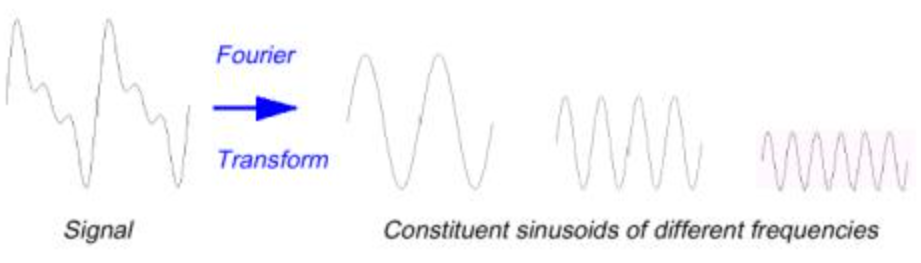
\includegraphics[scale=0.4]{img/wavelet.PNG}
\caption{Wavelet representation}
\label{fig:wavelet}
\end{figure}

A Wavelet is a time-localized wave-like oscillation; an example is shown in Figure \ref{fig:wavelet}. Scale and location are the two most basic features of wavelets. The scale (or dilation) of a wavelet determines how "stretched" or "squished" it is. This attribute has to do with how waves are characterized in terms of frequency. The wavelet's position in time is defined by its location (or space).

Then, the schema of features calculated is as follows. For each lead calculate:

\begin{enumerate}
    \item \textbf{Statistics}: Percentiles (5, 25, 50, 75, 95), mean, standard deviation and variance for the complete signals.
    
    \item Calculate \textbf{coefficients} of \textbf{Discrete Wavelet Transform (DWT)}. DWT gets local frequencies for the signals. The Coefficients are calculated using the function \texttt{wavedec} from the Python’s library \texttt{pywt}.
    
    \item For each \textbf{coefficient} of DWT calculate:
    \begin{itemize}
        \item \textbf{Statistics}: Percentiles (5, 25, 50, 75, 95), mean, standard deviation and variance.
        
        \item \textbf{Shannon’s entropy (same that entropy)}: It’s related to the “amount of information” of a variable. In other words, it measures the information of the distribution.
    \end{itemize}
\end{enumerate}


\subsubsection{Spectral features morphology}

\begin{equation} \label{spectral_feature_detail}
feature_s = l(Lead_i)\_c\_(Coefficient_j)\_(operation_k)
\end{equation}

Each 636 spectral feature is based on \textit{lead} as l, their \textit{coefficient} as c and \textit{operation} applied on it for example: mean, coefficient percentiles, standard deviation etc. Also, $lead_i$ represents ECG lead number from 00-11, $Coefficient_j$ represents a coefficient number from Discrete Wavelet Transform(there are 5 coefficients in total 1-5) and $operation_k$ represents the operation name like mean as average, standard deviation as std, variance as var, percentiles represents as n5(percentile 5), n25(percentile 25), n50(percentile 50), n75(percentile 75), n95(percentile 95) and entropy applied on coefficient get represented as c1-c5. At the end from each ECG lead, we get 53 features and in 53x12 we get 636 spectral features in total. Below in figure [\ref{fig:feature_importance}] names of features are represented by above represented [\ref{spectral_feature_detail}] morphology. 


\subsection{Exploratory Data Analysis (EDA)} \label{4eda}

Exploratory Data Analysis refers to the critical process of performing initial investigations on data to identify patterns, spot anomalies, test hypotheses, and check assumptions using summary statistics and graphical representations. It's important to initially comprehend the data before attempting to get as many insights as possible. EDA is all about making sense of data before getting their hands dirty with it. The major steps commonly examined in an EDA are shown in Figure \ref{fig:eda}.

\begin{figure}[H]
\centering
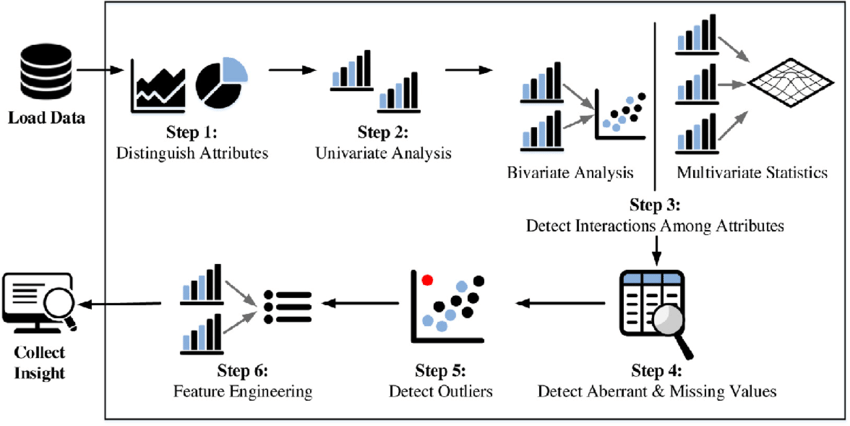
\includegraphics[scale=0.4]{img/EDAschema.PNG}
\caption{Schema of a EDA}
\label{fig:eda}
\end{figure}

\subsection{Unbalanced classes} \label{3unbclass}

One of the most difficult issues when training a model is modelling imbalanced data \cite{smote1}. When dealing with classification problems, the intended class balance is quite important. When a dataset has an uneven distribution of classes, the models attempt to learn only the dominant class, resulting in biased predictions.

One approach for addressing this issue is random sampling. Random resampling can be accomplished in two ways, each with its own set of benefits and drawbacks:

\begin{itemize}
    \item \textbf{Oversampling:} Replicating examples from the minority class.
    \item \textbf{Undersampling:} Deleting examples from the majority class.
\end{itemize}

To put it another way, both oversampling and undersampling include creating bias by selecting more instances from one class than from another. The prior is used to compensate for an imbalance that is already present in the data or that is likely to occur if a perfectly random sample is obtained \cite{smote2}. Because it makes no assumptions about the data, random sampling is a naive strategy. To minimize the data's influence on the Machine Learning algorithm, a fresh adjusted version of the data with a new class distribution is generated.

Random Oversampling and SMOTE were the two oversampling techniques chosen for this project. The synthetic Minority Oversampling Technique is a technique for creating synthetic samples for the minority class. Overcoming the problem of overfitting produced by random oversampling is easier with this method. It focuses on the feature space to generate new examples by interpolating between positive occurrences that are near in proximity.

\begin{figure}[H]
\centering
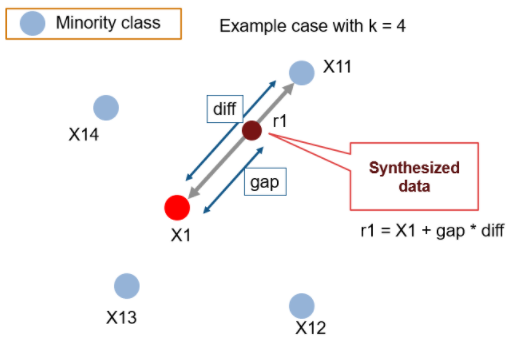
\includegraphics[scale=0.7]{img/SMOTE.PNG}
\caption{SMOTE process illustration}
\label{fig:smoteproc}
\end{figure}

SMOTE uses the k-nearest neighbour technique to create synthetic data. To make them follow the instructions below. \cite{smote1}:

\begin{enumerate}
    \item Find the nearest neighbours of the feature vector.
    \item Determine the distance between the two sample sites.
    \item At random, the distance is multiplied by an integer between 0 and 1.
    \item Find a new point on the line segment at the calculated distance.
    \item Rep the procedure for each of the feature vectors that were discovered.
\end{enumerate}

\subsection{Machine Learning Models} \label{3mlmodels}

Classifiers are the models provided in the following sections. These tools were created to determine which behaviours are more likely to be associated with various arrhythmia patterns. Each of these methods is widely utilized in various data-driven systems, and they have demonstrated useful behaviour in a variety of classifying tasks, including ECG classification (\ref{methods_ECG_class}).

The various versions of the dataset were created using Python Notebooks in Google Colab. This section will detail the key models that were tested and evaluated.

\subsubsection{Model 1 - (XGB) XG-Boost algorithm} \label{3model1}

The XG-Boost technique, which has proven to be effective in a variety of classification and regression problems, is the first attempt to classify ECG signals. The aforementioned algorithm has been used in a variety of sectors, including economics, credit rating, and health-related difficulties. The preceding are reasons to expect that such a strategy will be effective in the field of arrhythmia detection today.

XG-Boost is a decision-tree-based ensemble Machine Learning approach that uses gradient boosting (\cite{xgb1} \cite{xgb2}). When it comes to unstructured data prediction, \textit{Artificial Neural Networks} outperforms all other algorithms or frameworks (text, audio, pictures, etc.). However, for small-to-medium tabular data, such as the one utilized in this challenge, \textit{decision tree-based} algorithms are now rated best-in-class.

XG-Boost minimizes a loss function to provide an additive expansion of the objective function, similar to gradient boosting. Because XG-Boost is only interested in decision trees as base classifiers, the complexity of the trees is controlled using a variation of the loss function.

\begin{equation}
L = \sum_{i=1}^{n}{L(y_i,\hat{y_i})}+\sum_{k=1}^{K}{\Theta(p_k)}
\end{equation}
\begin{equation}
\Theta(w)=\gamma Z+\frac{1}{2} \lambda ||w||^2
\end{equation}

\noindent

The number of leaves on the tree is Z, and the leaf output scores are w (\cite{xgb2}). This loss function can be included in the split criterion of decision trees, resulting in a pre-pruning strategy. Trees with a greater $\gamma$ value are easier to understand. The amount of loss reduction gain required to separate an internal node is determined by $\gamma$ (\cite{xgb1}). Shrinkage is a regularization parameter in XG-Boost that decreases the step size in the additive expansion. Finally, other techniques such as tree depth can be utilized to keep the trees from becoming too complex. As a result of lowering tree complexity, the models are trained faster and need less storage space.

\subsubsection{Model 2 - (Catboost) Catboost} \label{3model2}

The second candidate for predicting the arrhythmia type for ECG is the Catboost algorithm. The latter is a decision tree gradient boosting technique. It was created by Yandex (with its final version in 2017) researchers and engineers and is used by Yandex and other firms such as CERN, Cloudflare, and Careem taxi for search, recommendation systems, personal assistant, self-driving cars, weather prediction, and many other activities. Anyone can use it because it is open-source.

\begin{figure}[H]
\centering
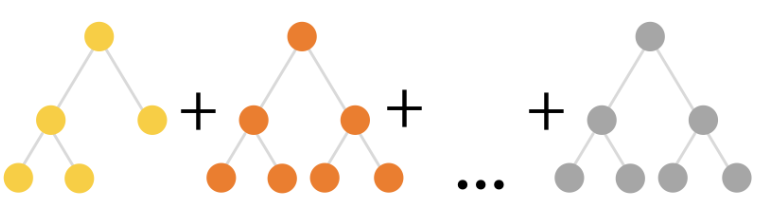
\includegraphics[scale=0.6]{img/catboost.PNG}
\caption{Catboost (decision trees) illustration}
\label{fig:catboost}
\end{figure}

The implementation of ordered boosting \cite{catboost}, a permutation-driven alternative to the conventional approach, and a novel technique for processing category characteristics are two key algorithmic innovations offered in CatBoost. Both strategies were developed to combat a prediction shift induced by a specific type of target leakage found in all current gradient boosting algorithm implementations.

\subsubsection{Model 3 - (DNN) Deep Neural Networks} \label{3model3}

A Deep Neural Network is another method for predicting ECG diagnosis. A DNN is a set of algorithms that attempts to recognize relationships in a batch of data by mimicking how the human brain functions.

In this context, deep neural networks refer to organic or artificial systems of neurons (\cite{ann1}). Deep neural networks can adapt to changing input and produce the best possible result without requiring the output criteria to be modified because they can adapt to changing input. Neural networks, an artificial intelligence-based concept, are swiftly gaining popularity in the development of trading systems.

Neural networks aid in time-series forecasting, algorithmic trading, securities classification, credit risk modelling, and the generation of proprietary indicators and price derivatives in the financial world (\cite{ann2} \cite{ann3}). The deep neural network of the human brain is akin to a neural network. A "neuron" in a deep neural network is a mathematical function that collects and categorizes data according to a set of rules. The network closely resembles curve fitting and regression analysis, two statistical methods.

\begin{figure}[h!]
\centering
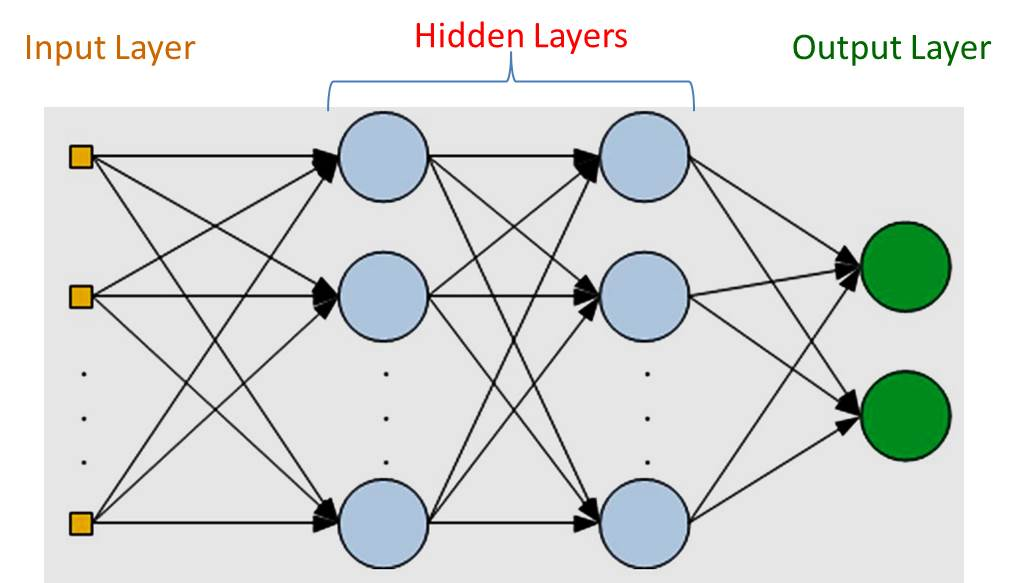
\includegraphics[scale=0.6]{img/Multilayer-Perceptron.jpg}
\caption{Deep Neural Network (Multi-layer Perceptron) schema}
\label{fig:mlp}
\end{figure}

Perceptrons are grouped in interconnected layers in a multi-layered perceptron (MLP) \cite{ann3}, as indicated in Figure \ref{fig:mlp} . The input layer is responsible for collecting input patterns. In the output layer, input patterns can be mapped to classifications or output signals. Hidden layers fine-tune the input weightings until the neural network's margin of error is as little as possible. Hidden layers are supposed to deduce salient elements from input data that can predict outcomes. This is how feature extraction works, and it's similar to how statistical methods such as principal component analysis function (\cite{ann3}).

\subsubsection{Model 4 - (LSTM) Long-Short Term Memory} \label{3model4}

Long short-term memory networks are a type of Deep Learning network. It's a class of recurrent neural networks (RNNs) that can learn long-term dependencies, which is useful for solving sequence prediction issues. Apart from single data points like photos, LSTM has feedback connections, which means it can process the complete sequence of data.

\begin{figure}[H]
\centering
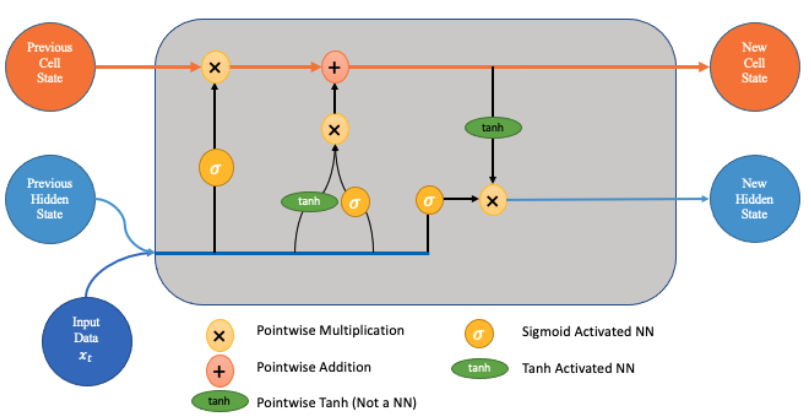
\includegraphics[scale=0.5]{img/lstm.png}
\caption{LSTM general schema}
\label{fig:lstm}
\end{figure}

An LSTM model's primary role is played by a memory cell called a 'cell state,' which maintains its state across time. The horizontal line that runs through the top of the diagram below represents the cell state. It can be compared to a conveyor belt on which data just passes, unmodified \cite{lstm}.


\subsubsection{Model 5 - Challenge Team 2 - ResNet with an SE layer\cite{second_team} } \label{3model5}

Challenge team 2 designed a modified ResNet with larger kernel sizes that model long-term dependencies. They embedded a Squeeze-And-Excitation layer into the modified ResNet to learn the importance of each lead adaptively. 

After obtaining the input signals, they designed ResNet to assign the 12-lead ECG recordings to the 24 diagnostic classes. 

\begin{figure}[H]
\centering
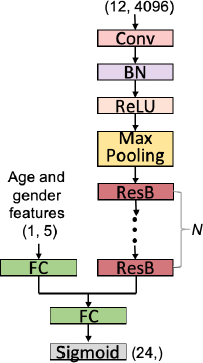
\includegraphics[scale=0.5]{img/team_two_network.png}
\caption{The proposed network architecture.}
\label{fig:team_two_network}
\end{figure}


As shown in [\ref{fig:team_two_network}] the improved ResNet consists of one convolutional layer followed by N = 8 residual blocks (ResBs), each of which contains two convolutional layers and a squeeze and excitation (SE) block (Fig. 2). Since some samples have multiple classes of 27 clinical diagnoses, instead of using the softmax function in a traditional classification problem, they assumed that each class was independent and used the sigmoid function for each output neurons to cope with this multi-task problem.

The first (convolutional) layer and the initial two ResBs units have 64 convolution filters. The number of filters increases by a factor of two for every second ResB unit. The feature dimension is halved after the max pooling layer, and the third, fifth, and seventh ResBs.

The improved ResNet has four modifications from the original ResNet \cite{he2015delving}. First, they modified the final fully connected (FC) layer to incorporate patient age and gender. These two features were passed through another FC layer with 10 neurons before inclusion in the final layer. Second, they used a relatively large kernel size of 15 in the first convolutional kernel, and a large kernel size equal to 7 in the latter convolutional kernels. Previous work has shown that large kernel sizes are more helpful for networks to learn meaningful features \cite{hannun2019cardiologist}. 


\begin{figure}[H]
\centering
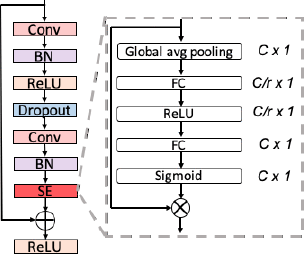
\includegraphics[scale=0.5]{img/team_two_network_2.png}
\caption{The proposed network architecture.}
\label{fig:team_two_network_2}
\end{figure}

Third, as shown in [\ref{fig:team_two_network_2}], they added a dropout layer with a dropout rate of 0.2 between two convolutional kernels in each ResB to reduce the likelihood of overfitting. Finally, They added a SE block into each ResB depicted in [\ref{fig:team_two_network_2}]. The SE block has been to model channel inter-dependencies, and in this case, they incorporate it to model the spatial relationship between the ECG channels. The SE block, introduced by \cite{Hu_2018_CVPR} uses a multi-layer perceptron (MLP) with one hidden layer to calculate the importance of the channels. The parameter r = 16 in Fig. 2 denotes the reduction factor, which controls the capacity of the MLP.


\subsubsection{Model 6 - Challenge Team 20 - A hybrid model (CNN + Rule Based )\cite{second_team} } \label{3model6}

Team 20 developed a hybrid model combining a rule-based algorithm with different deep learning architectures. They compared two different Convolutional Neural Networks, a Fully Convolutional Neural Network and an Encoder Network, a combination of both, and with the addition of another neural network using age and gender as input. Two of these combinations were finally combined with a rule-based model using derived ECG features. 

\textbf{CNN Architectures:}

As a starting point for classifying the ECG signals, they employed FCN and Encoder types of CNN models as described in \cite{ismail2019deep}. Two models were tested without any modifications to the architecture other than changing the input and output layers to fit our input data and output classes. All output layers of each model used a Sigmoid activation function.

To make use of the provided age and gender data, a simpler neural network model with 2 inputs, one hidden layer of 50 units, and 2 outputs in the final layer was added. This new model was combined with our FCN and Encoder models by concatenation of the last layer of the CNNs.

Age and gender data were passed into the simple neural network as integers, but in some information files, the age of the patient was not given and was assigned a value of -1. The gender data was transformed into integers, where a male was set equal to 0, a female equal to 1, and an unknown was set to 2.

The two CNN models (FCN and Encoder) were combined as parallel models, concatenated on the second last layer. This model was tested with and without a parallel dense layer1.

\textbf{Rule-Based Model}

The rule-based algorithm used the raw ECG signal, without any padding or truncating, as input. R-peak detection \cite{4122029}, and heart rate variability (HRV) analysis was programmed to add relevant derived features to the algorithm. An HRV score was obtained by computing the root mean square of successive differences between normal heartbeats (RMSSD) using the detected R-peaks as timing indicators of each heartbeat.

The rule-based algorithm was able to classify eight different diagnoses: atrial fibrillation, bradycardia, low QRS-complex, normal sinus rhythm, pacing rhythm, sinus arrhythmia, sinus bradycardia, and sinus tachycardia.

The rule-based algorithm performed classification independent of the deep learning models. If there was disagreement between the rule-based algorithm and the CNN model, the rule-based algorithm overwrote the classification from the CNN model.


\subsection{Metrics} \label{3metrics}

It is vital to create metrics that will assist in determining whether a model is better than others to determine whether it is better than others. There are explanations for each of the metrics used in the following sections.


\subsubsection{Confusion Matrix} \label{4confmatrix}

A confusion matrix, like the one shown in table \ref{table:confmatr}, demonstrates how well a classification model works on test data for which the true values are known (\cite{metrics2}). The confusion matrix is simple in itself, but the related nomenclature can be confusing. In the following examples, I've created a hypothetical target variable called "Diagnose A" with the values "Yes" (if the recording belongs to that diagnosis) and "No" (if the recording does not belong to that diagnosis).


\begin{table}[H]
\centering
\begin{tabular}{ |p{4cm}||p{4cm}||p{4cm}|  }
 \hline
 \multicolumn{3}{|c|}{\textbf{Actual Class}} \\
 \hline
 \textbf{Predicted Class}  & Diagnose A - YES = 1 & Diagnose A - NO = 0\\
 \hline
 Diagnose A - YES = 1 & True Positives (\textbf{TP})  & False Positives (\textbf{FP}) \\
 Diagnose A - NO = 0 & False Negatives (\textbf{FN})  & True Negatives (\textbf{TN}) \\
 \hline
\end{tabular}
\caption{Confusion Matrix representation}
\label{table:confmatr}
\end{table}

Here is an explanation for each of the matrix's elements to understand the preceding terminology (\cite{metrics2} \cite{metrics1}).

\begin{itemize}
    \item \textit{True negatives (TN):} The model predicted they wouldn't have diagnosed A, and they don't.
    \item \textit{True positives (TP):} These are examples when the model predicted yes (the recording has the diagnose A), and they don't.
    \item \textit{False positives (FP):} The model projected that they would have diagnosed A, but they don't. (This is also referred to as a "Type I error.")
    \item \textit{False negatives (FN):} The model anticipated that they would not have diagnosed A, yet they do. (This is often referred to as a "Type II error.")
\end{itemize}

\subsubsection{Accuracy} \label{4accuracy}

\begin{equation}
    Accuracy = \frac{TP+TN}{TP+FP+FN+TN}
\end{equation}

The most basic performance metric is accuracy, which is defined as the proportion of correctly predicted observations to all observations. If a model is correct, one would assume it is the best. Yes, accuracy is a relevant measure when the datasets are symmetric and the number of false positives and false negatives is about equal.

Imagine the case when the training set contains 98 percent samples of class A and $2\%$ samples of class B, for example. The model may thus easily attain a $98\%$ training accuracy by simply guessing every training sample that belongs to class A. When the same model is tested on a test set that contains $60\%$ class A samples and $40\%$ class B samples, the test accuracy reduces to $60\%$. As a result, classification accuracy is poor, but it gives the image of great accuracy.

Then, when the cost of misclassification of minor class samples becomes significant, (\cite{metrics1}) the true issue appears. The cost of failing to diagnose, for example, a sick person's ailment is significantly greater than the expense of submitting a healthy person to additional tests when dealing with a rare but lethal disorder.

\subsubsection{Precision} \label{4precision}
\begin{equation}
    Precision = \frac{TP}{TP+FP}
\end{equation}

Precision \cite{metrics2} is the ratio of accurately predicted positive observations to total expected positive observations. This measure answers the question of how many of the drivers who were identified as drowsy drove. Precision is linked to a low false-positive rate.

Precision is a good statistic to employ when the costs of False positives are high. Take, for example, the identification of email spam. In email spam detection, a false positive happens when an email that is not spam (actual negative) is wrongly identified as spam (predicted spam). If the precision of the spam detection model is low, the email user may miss important emails.

\subsubsection{Recall} \label{4recall}
\begin{equation}
    Recall = \frac{TP}{TP+FN}
\end{equation}

Recall \cite{metrics2} is the ratio of successfully predicted positive observations to all observations in the actual class. It's meant to answer the question of how many drivers who slept were labelled as such.

In the case of identifying sick patients, for example, if a sick patient (Actual Positive) conducts the test and is predicted to be healthy (Predicted Negative). The cost of a False Negative will be quite high if the condition is infectious.

\subsubsection{F1 Score} \label{4F1}
\begin{equation}
    F1 Score = \frac{2*(Recall * Precision)}{(Recall + Precision)}
\end{equation}

The F1-Score is the weighted average of Precision and Recall. As a result, both false positives and false negatives are taken into account in this score. F1 is often more valuable than accuracy, despite the fact that it is less intuitive (\cite{metrics1} \cite{metrics2}). This is especially true if the class distribution is unequal. When the costs of false positives and false negatives are equal, accuracy works well. If the cost of false positives and false negatives differs significantly, it is best to evaluate both Precision and Recall.

\subsubsection{Overall index} \label{4overallindex}

As a final metric, I introduced the use of the mean value of Accuracy, Precision, Recall and F1-Score. With the latter, it is possible to check with only one metric the overall behaviour of the classifiers.

% \subsection{Fine tuning hyper parameters} \label{3finetuning}

% Models for machine learning are made up of two sorts of parameters:

% \begin{itemize}
%     \item - \textbf{Hyper parameters:} Those are all the parameters that the user can specify freely before beginning training (e.g. number of estimators in XG-Boost).
%     \item - \textbf{Model parameters:} Those are learned during model training instead (e.g. weights in Neural Networks).
% \end{itemize}

% The model parameters are learned during training and define how to use input data to produce the desired output. Hyperparameters, on the other hand, govern how the model is structured. Tuning Machine Learning models is an example of an optimization problem. There are a set of hyperparameters, and the objective is to determine the best combination of their values to find the minimum (for example, loss) or maximum (for example, accuracy) of a function. 

% This is especially significant when evaluating the performance of multiple Machine Learning models on a dataset. Comparing an XG-Boost model with the best hyperparameters against a Neural Network model that has not been optimized would be unfair.

% \begin{figure}[H]
% \centering
% 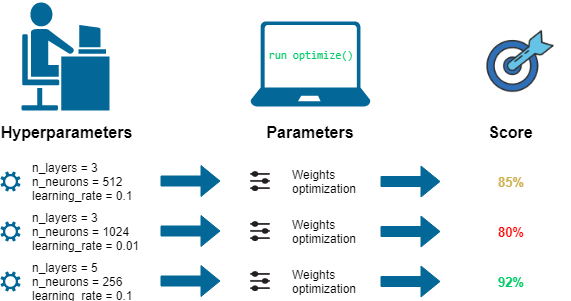
\includegraphics[scale=0.5]{finetuning.png}
% \caption{Example hyper parameters fine tuning }
% \label{fig:finetuning}
% \end{figure}


% Along with this thesis, there are two main approaches used to find the optimal hyperparameters for the selected methods: Grid search and Random Search.

% \subsubsection{Grid Search} \label{31gridsearch}

% One can put up a grid of hyperparameters in Grid Search and train/test the model on all the potential combinations. To determine the parameters to utilize in Grid Search, one may now look at several possible ranges and create a grid based on them to see if a better combination can be found. The scikit-learn \textit{GridSearchCV()} function can be used to implement Grid Search in Python.

% \subsubsection{Random Search} \label{31randomsearch}

% In Random Search, a grid of hyperparameters is created, and the model is trained/tested using only a random mix of these hyperparameters. In addition, Cross-Validation on the training set is an option. When doing Machine Learning tasks, the dataset is usually divided into training and test sets. This is done so that the model may be tested after it has been trained (in this way, it is possible to check its performances when working with unseen data). To ensure that our model is not overfitting the data, we divide the training set into K other divisions using Cross-Validation.


\section{Edge computing(EC) fundamentals} \label{4ecomfun}

\subsection{Definition}
Edge computing is a distributed computing paradigm that brings computation and data storage closer to the sources of data. This is expected to improve response times and save bandwidth. It is an architecture rather than a specific technology. It is a topology- and location-sensitive form of distributed computing.

Edge computing is primarily concerned with transmitting data among the devices at the edge, closer to where user applications are located, rather than to a centralized server (see \ref{fig:ec_fundamentals}). The edge node (or edge client, edge device) is usually the resource-constraint device that the end user uses and it is geographically close to the nearest edge server, who has abundant computing resources and high bandwidth communicating with end nodes. When the edge server requires more computing power, it will connect to the cloud server. The most important consequences of this architecture are twofold: latency is dramatically reduced as data does not need to travel as far, and bandwidth availability improves significantly, as the user is no longer relying on sharing a single traffic lane to transfer their data. Indeed, this new computing paradigm offers great cost savings for companies that do not have the resources to build dedicated data centers for their operations. Instead, engineers can build a reliable network of smaller and cheaper edge devices. \cite{fedrated_learning_as_edge_computing}


\begin{figure}[H]
\centering
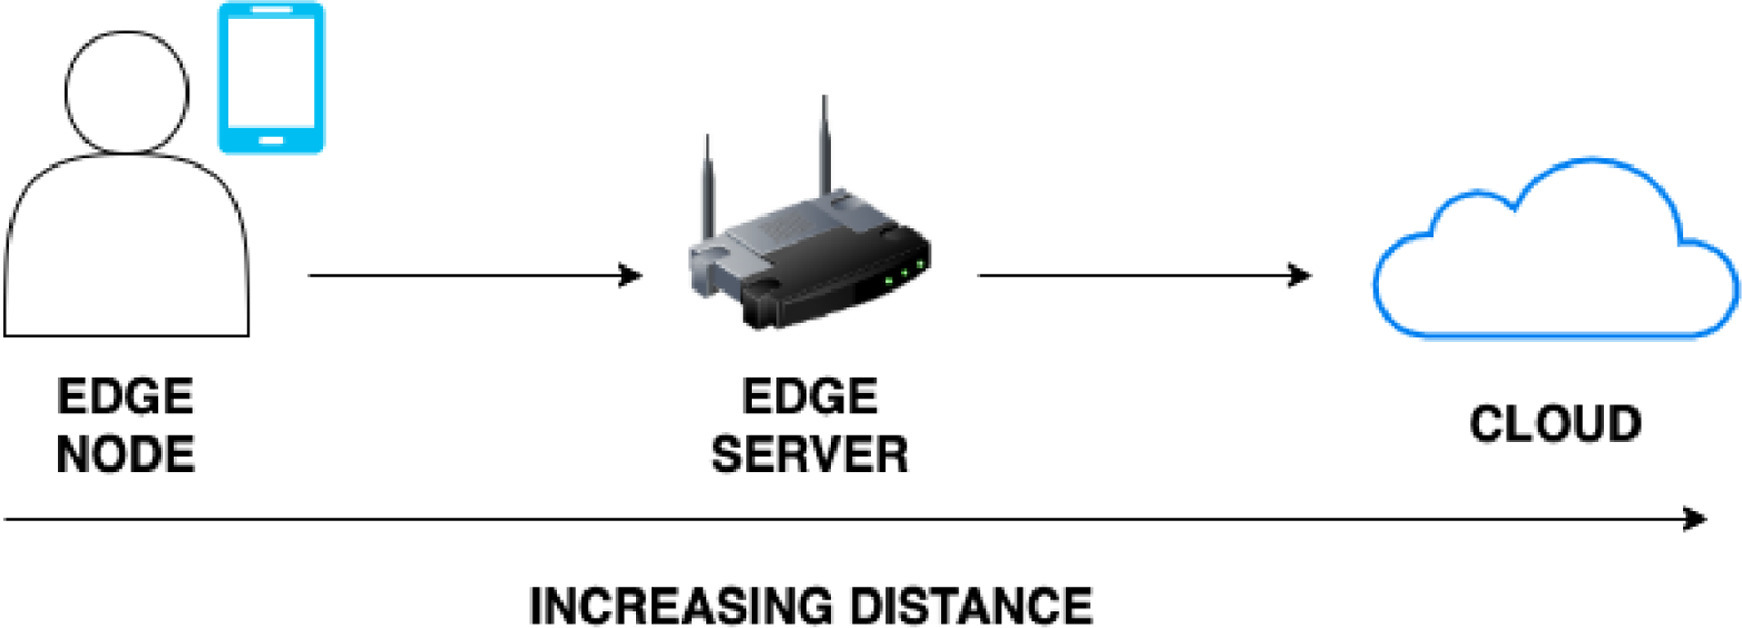
\includegraphics[scale=0.6]{img/edge_computing_main_pic.jpg}
\caption{Edge Computing Overview}
\label{fig:ec_fundamentals}
\end{figure}


In addition, federated learning has been discussed a lot recently. It is a collaborative machine learning framework allowing devices from different resources with different private datasets working together to study and train a global model. Federated learning can not only collaborate the computational resources from different devices but also preserve privacy at the same time.


Given the common features of both edge computing and federated learning, edge computing is a naturally suitable environment to apply the federated learning framework. Therefore, edge federated learning is more and more appealing in both academic research and industry in recent days. Here, we first have a brief introduction to edge computing and federated learning respectively and discuss them in detail later. 

\subsection{Reasons for Edge Computing:}

There are a set of key reasons why industry executives are transitioning from 
a traditional cloud-based model to edge computing platforms. The two major factors that were already discussed beforehand are low latency and high bandwidth \cite{satyanarayanan2017emergence}. However, the edge also provides for greater security. For example, sending data to an edge device will give any potential attackers less time to launch an attack as compared to the cloud simply because the latency is lower. Moreover, attacks like DDoS that would normally be debilitating in a cloud-based environment are rendered almost harmless in an edge computing environment because the affected edge devices can be removed from the network without hampering the overall functionality of the network as a whole. Of course, this also means that edge networks are much more reliable as they do not have a single point of failure. As discussed briefly beforehand, edge networks are much more easily scalable because the devices have much smaller footprints. Indeed, a scale-out strategy of scalability rather than a scale-up one offers companies a very attractive way of getting good performance at a low cost. Moreover, some of these edge devices or edge data centers may not even need to be built from scratch by any one company. Different stakeholders can partner up to share the resources from the already existing IoT devices in the edge network.


\subsection{EC Operating Principles:}

To deliver these benefits to end-users, engineers have relied on a common set of key operating principles when building edge computing systems \cite{khan2019edge}:

\textbf{Mobility}: For applications like self-driving cars, the edge devices have to accommodate a constantly moving end-user without sacrificing latency or bandwidth. Some approaches solve this problem by positioning edge devices on the roadside.


\textbf{Proximity}: To deliver low latency guarantees, the edge devices must be positioned as close as possible to the end users. This could mean performing computation directly at the edge device or investing in a local edge computing data center that is close to the end-user.

\textbf{Coverage:} For edge computing to become ubiquitous, network coverage must be far-reaching. Thus, the exact distribution of nodes in an edge computing framework is imperative to achieving an optimal user experience. Of course, a dense distribution is preferred, but this must be balanced with cost constraints.



\section{Federated learning (FL) fundamentals} \label{4fedlea}

\subsection{Definition}
Federated learning (FL) is a machine learning technique for training machine learning models cooperatively on several devices or local servers in a decentralized way, preserving data privacy and data ownership for the device/server owner \cite{fl8}. FL is extremely advantageous for highly decentralized healthcare data, especially with the growing prevalence of IoT devices for continuously capturing data and monitoring health.


\begin{figure}[H]
\centering
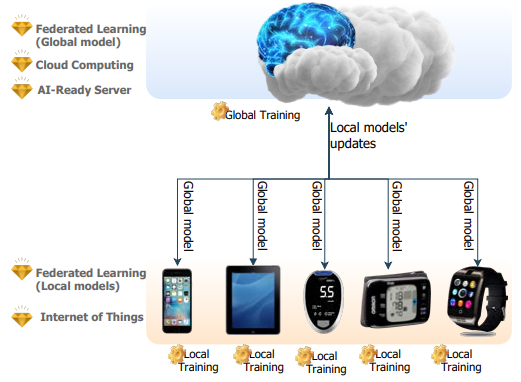
\includegraphics[scale=0.6]{img/fl_overview.png}
\caption{FL framework Overview}
\label{fig:fl_overview}
\end{figure}

Figure \ref{fig:fl_overview} depicts a high-level view of the framework and how the technologies will interact together. The IoT devices will collect data from users and train a local deep learning model that is a copy of a global model that was previously received. Following the completion of the local training phase, the models will collaborate to train a global model utilizing their updates rather than the raw data provided by the users. These model updates indicate changes in the weights of the models during the training process and do not reflect any private or personal information about the users.

All participating models will send updates to a cloud server, where they will be compiled and used to train the global model \cite{fl2} \cite{fl3}. Each device will receive a new copy of the updated global model once the global model training procedure is completed. As a result, the models will be trained and updated regularly without sharing any personal information. As a result, the framework will support an IoT-based decentralized architecture in which models are spread among IoT devices without the need for a centralized server to operate the model and serve users. It will also protect users' privacy by processing and analyzing their data on IoT devices without disclosing it.

\subsection{FL types}

FL is divided into five categories \cite{fl26_types} based on data partitioning, machine learning models (ML Models), privacy mechanisms, communication architecture, and federation scale.

\subsubsection{Data Partitioning}

The datasets of various clients share the same properties in \textbf{Horizontal data partitioning} \cite{fl25}, however, there is limited sample space intersection. All FL architectures use horizontal partitioning the most. Aggregation at the server is made easier by the fact that a standard model can be used for all clients; FedAvg is typically used for aggregation. A dataset containing ONLY breast cancer patients from a specific hospital would be simple to comprehend example. 

\begin{figure}[H]
\centering
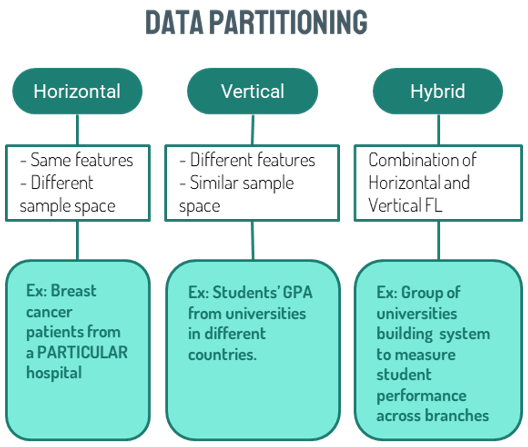
\includegraphics[scale=0.5]{img/fl_data_partition.png}
\caption{Data partition-based FL types}
\label{fig:fl_data_partition}
\end{figure}

When clients are exposed to distinct feature spaces but the same or similar sample space, \textbf{Vertical Data Partitioning} comes into play. Entity alignment algorithms are utilized to find overlapping samples among the client data, and this overlapped data is used for training \cite{fl26_types}. A dataset of students' GPAs obtained from institutions across the globe is a nice example. The feature space, which includes the grading scale and evaluation measure, is distinct.

Horizontal and vertical data partitioning are combined in \textbf{Hybrid Data Partitioning}. A set of universities intending to develop an FL System to assess student achievement across branches is an easy to comprehend case for hybrid partitioning.

\subsubsection{ML models}

The issue statement and dataset are frequently used to determine the machine learning models to use \cite{fl26_types}. One of the most widely used models is neural networks (NN). Apart from NNs, decision trees are also used, as they are highly efficient and simple to understand. Models can be \textbf{homogeneous} or \textbf{heterogeneous} in a FL system. 

\begin{figure}[H]
\centering
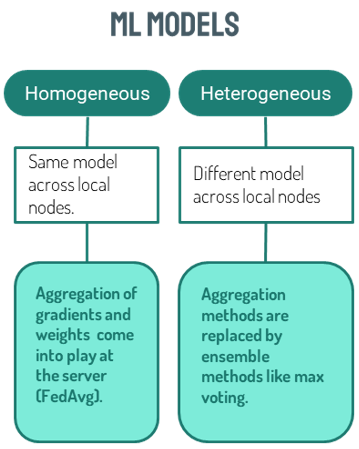
\includegraphics[scale=0.5]{img/fl_mlmodels.png}
\caption{ML models-based FL types}
\label{fig:fl_mlmodels}
\end{figure}

In the case of the former, all clients use the same model, while the server uses gradient aggregation. In the latter instance, however, there is no possibility of aggregating because each client has a unique model. Aggregation methods are substituted with ensemble methods like max voting at the server in the case of heterogeneous models \cite{fl26_types}.

\subsubsection{Privacy Mechanisms}

The most controversial part of FL is how it deals with privacy. The main concept is to prevent client information from leaking out. The server may decipher the data of clients without encryption by applying learning gradients. As a result, it's critical to hide the gradients. Differential privacy and cryptographic approaches are commonly used to address privacy concerns in FL systems.

\begin{figure}[H]
\centering
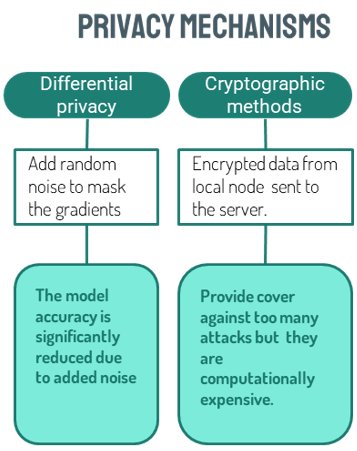
\includegraphics[scale=0.5]{img/fl_privacy_methods.png}
\caption{Privacy Mechanisms-based FL types}
\label{fig:fl_privacy_methods}
\end{figure}

\textbf{Differential privacy} is a technique for hiding gradients by adding random noise to data or model parameters. Due to the extra noise, this strategy has a considerable negative in terms of model accuracy.

In FL systems, \textbf{cryptographic approaches} such as homomorphic encryption and safe multi-party computation is commonly used. The process is straightforward: clients send encrypted data to the server, the server processes the data, and then the encrypted output is decrypted to obtain the final result. Even though these methods protect against a wide range of threats, they are computationally intensive.

\subsubsection{Architecture}

There are two types of FL system architecture: centralized and decentralized. Both types of architecture work in the same way; the only difference is in client-server communication. We have a second model that acts as a server in a \textbf{centralized architecture}, and all parameter updates are done in this global model. 

\begin{figure}[H]
\centering
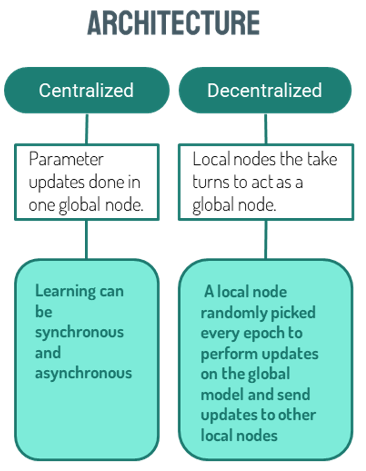
\includegraphics[scale=0.5]{img/fl_architecture.png}
\caption{Architecture-based FL types}
\label{fig:fl_architecture}
\end{figure}


In a \textbf{decentralized design}, on the other hand, clients take turns acting as servers. Every epoch, a client is chosen at random to make global model changes and send the global model to other clients.

\subsubsection{Scale of Federation}

The scale of the federation can be divided into two types: cross-silo and cross-device. To grasp the distinction between the two, relate cross-silo with organizations and cross-devices with mobiles. When using \textbf{cross-silo}, the number of clients is usually minimal, but they have a lot of computing power. 

\begin{figure}[H]
\centering
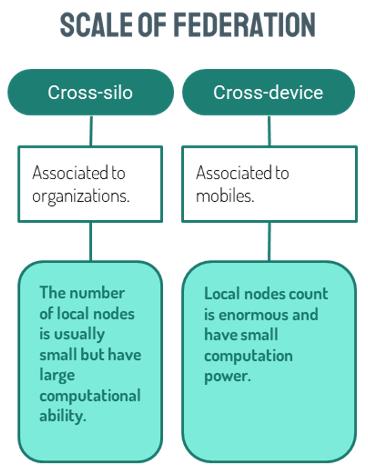
\includegraphics[scale=0.5]{img/fl_scale.png}
\caption{Scale of federation-based FL types}
\label{fig:fl_scale}
\end{figure}

Regarding \textbf{cross-device}, the number of clients is enormous, but their computing power is limited. Another consideration is reliability: while we can rely on organizations (cross-silo) to be ready to train at all times, this is not the case with mobile phones (cross-devices). There's a chance that a bad network will make the gadget unavailable.

\subsection{Advantages and disadvantages}

FL has a lot of advantages over traditional, centralized systems \cite{fl27_adv_disadv}. Some of the most remarkable upper hands of FL are:

\begin{itemize}
    \item \textbf{Data security}: Keeping the training dataset on the devices eliminates the need for a data pool for the model.
    \item \textbf{Data diversity}: Companies may be unable to merge datasets from diverse sources due to challenges other than data security, such as network unavailability in edge devices. Federated learning makes it easier to access diverse data, even when data sources can only interact at particular periods.
    \item \textbf{Continuous learning in real time}: Models are continuously enhanced utilizing client input, eliminating the requirement to aggregate data for continuous learning.
    \item \textbf{Technology efficiency}: Because federated learning models do not require a single complex central server to evaluate data, this technique requires less complex hardware.
\end{itemize}

On the other hand, FL needs to deal with some relevant challenges. The most common are:

\begin{itemize}
    \item \textbf{Investment requirements}: FL models may necessitate frequent communication between nodes, which may necessitate an investment. This means that high bandwidth and storage capacity are among the system requirements.
    
    \item \textbf{Data Privacy}: In FL, data is not collected on a single entity/server; instead, numerous devices are used to collect and analyze data. Even though only models, not raw data, are transferred to the central server, models can be reverse engineered to identify client data, thereby increasing the attack surface. Differential privacy, secure multiparty computation, and homomorphic encryption are examples of privacy-enhancing technologies that can be utilized to improve the data privacy capabilities of federated learning.
    
    \item \textbf{Performance limitations}: In FL, models from several devices are combined to create a superior model. Device-specific factors may hinder the generalization of models from some devices, lowering the accuracy of the model's next generation. Researchers investigated scenarios in which one of the federation's members could use secret backdoors in the joint global model to intentionally attack others.
\end{itemize}

\subsection{Proposed approach} \label{proposed_approaches}

After understanding the theory and characteristics behind the FL techniques I proposed an approach while using the PhysioNet 2020 datasets.

It's structure is explained in figure [\ref{fig:fl_approach}].

\begin{figure}[H]
\centering
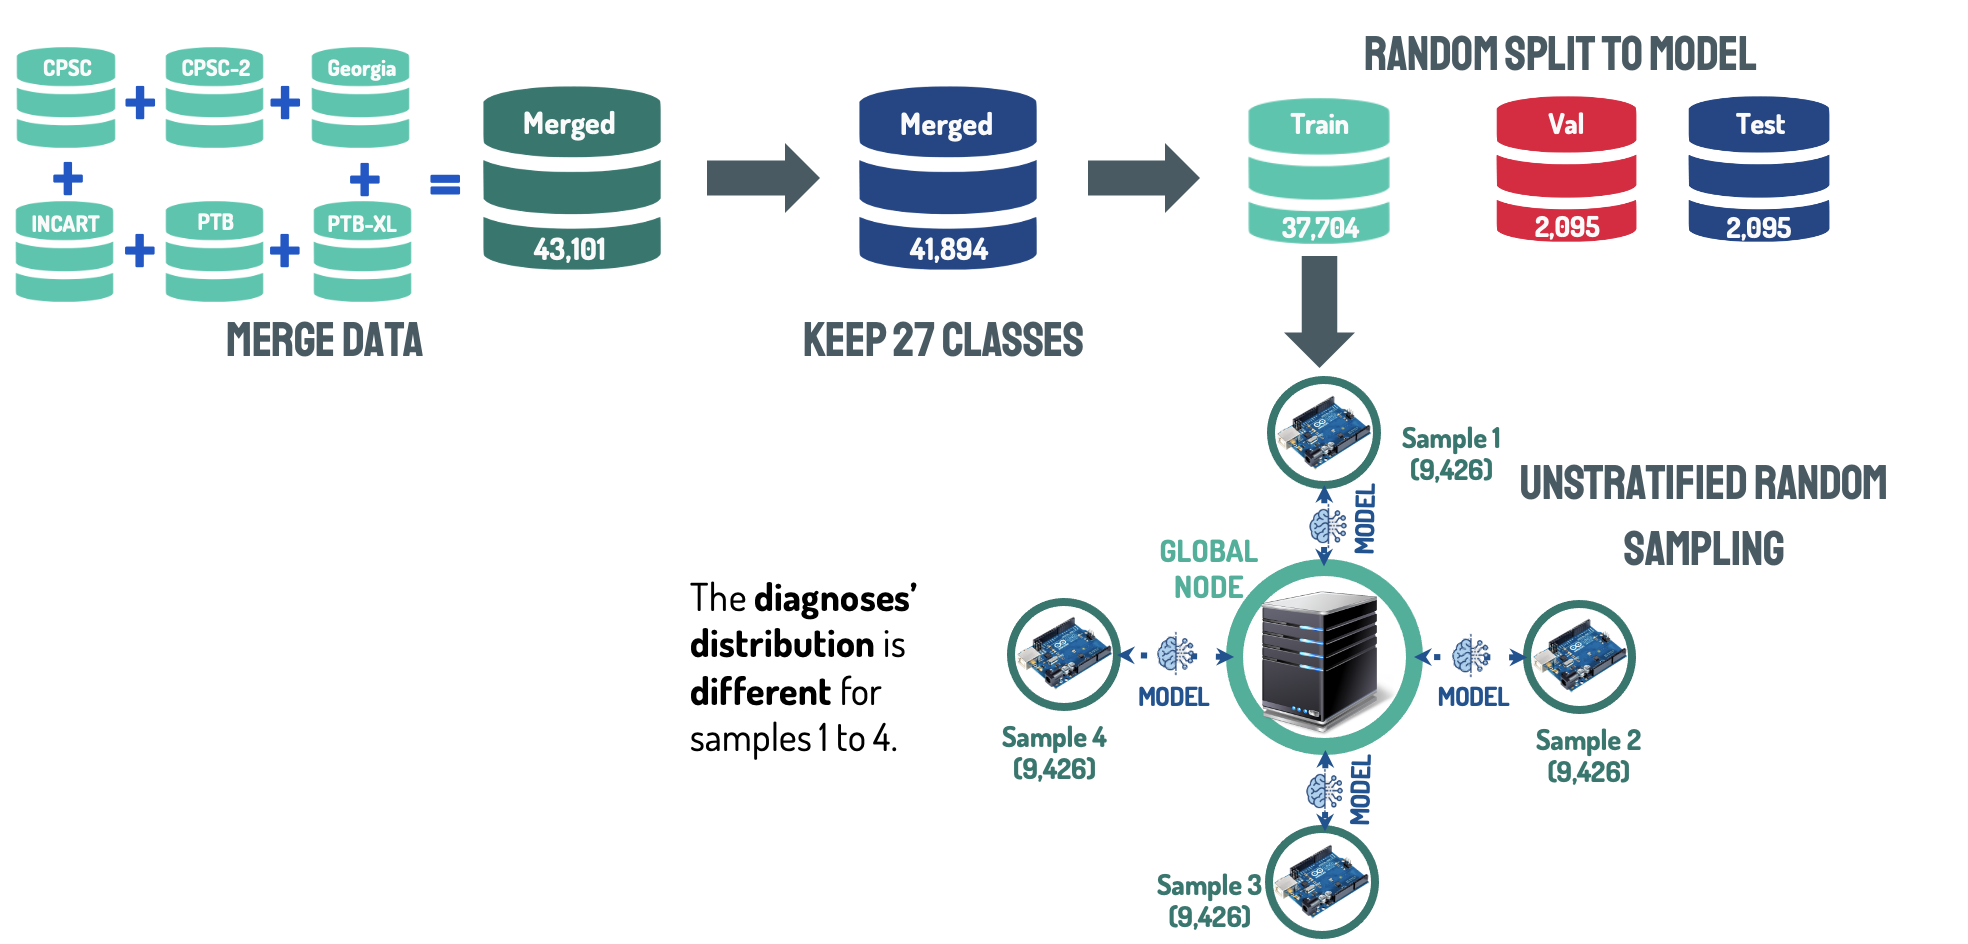
\includegraphics[scale=0.4]{img/fl_approach.png}
\caption{Proposed approach}
\label{fig:fl_approach}
\end{figure}

In the above approach, I combined all six datasets (additional information here \ref{5dataset}) into a single dataset including 43,101 recordings. I came up with 41,894 after utilizing the methodology described in figure \ref{fig:fl_approach} (filtering out the non-representative classes). After that, I divided the data into train, validation, and test datasets at random. Later, I used an Unstratified random sampling (with replacement) method to acquire four separate samples from the original data. As a result, each sample has a varied distribution of labels (diagnoses).

\newpage 

\section{Model conversion process} \label{4mconverionp}

As depicted in \ref{fig:framework_used_by_2020_teams} , most of teams used \textbf{Pytorch} during the challenge implementation. As I am going to use Tensorflow as a primary framework and later Tensorflow Lite for using them on mobile phones or IoT devices. Before going to the conversion process itself let's look at the fundamentals of Pytorch, Tensorflow and Tensorflow Lite.


\subsection{Pytorch:}
PyTorch is an open source machine learning framework based on the Torch library, used for applications such as computer vision and natural language processing, primarily developed by Meta AI. It is free and open-source software released under the Modified BSD license. Although the Python interface is more polished and the primary focus of development, PyTorch also has a C++ interface.

Several pieces of deep learning software are built on top of PyTorch, including Tesla Autopilot, Uber's Pyro, Hugging Face's Transformers, PyTorch Lightning, and Catalyst.

\textbf{Features:}
\begin{enumerate}
  \item Tensor computing (like NumPy) with strong acceleration via graphics processing units (GPU)
  \item Deep neural networks built on a tape-based automatic differentiation system.
\end{enumerate}

\subsection{Tensorflow:}

TensorFlow is a free and open-source software library for machine learning and artificial intelligence. It can be used across a range of tasks but has a particular focus on the training and inference of deep neural networks.

TensorFlow was developed by the Google Brain team for internal Google use in research and production. The initial version was released under the Apache License 2.0 in 2015. Google released the updated version of TensorFlow, named TensorFlow 2.0, in September 2001. TensorFlow can be used in a wide variety of programming languages, most notably Python, as well as Javascript, C++, and Java. This flexibility lends itself to a range of applications in many different sectors.

\textbf{Features:}

\begin{enumerate}
  \item \textit{AutoDifferentiation} is the process of automatically calculating the gradient vector of a model concerning each of its parameters. 
  \item TensorFlow includes an \textit{eager execution} mode, which means that operations are evaluated immediately as opposed to being added to a computational graph which is executed later.
  \item In both eager and graph executions, TensorFlow provides an API for distributing computation across multiple devices with various distribution strategies. 
  \item To train and assess models, TensorFlow provides a set of \textbf{loss} functions (also known as cost functions).
\end{enumerate}

There are several other features Tensorflow framework provides in which Tensorflow Lite is one of them. 

\subsection{Tensorflow Lite:}
TensorFlow Lite is a set of tools that enables on-device machine learning by helping developers run their models on mobile, embedded, and edge devices.
\break\break
\textbf{Features:} 

\begin{enumerate}
  \item Optimized for on-device machine learning, by addressing 5 key constraints: latency (there's no round-trip to a server), privacy (no personal data leaves the device), connectivity (internet connectivity is not required), size (reduced model and binary size) and power consumption (efficient inference and a lack of network connections).
  \item Multiple platform support, covering Android and iOS devices, embedded Linux, and microcontrollers.
  \item Diverse language support, which includes Java, Swift, Objective-C, C++, and Python.
  \item High performance, with hardware acceleration and model optimization.
  \item End-to-end for common machine learning tasks such as image classification, object detection, pose estimation, question answering, text classification, etc. on multiple platforms.
\end{enumerate}

\subsection{Conversion steps:}

As we have seen above definitions and features of different frameworks. Let's now look at how we can convert the Pytorch model to TensorFlow lite. 

\begin{enumerate}

\item First we train the model using a dataset or get a trained model from any challenges team as most of them already stored them in .pt or .pth format. 
\break We can utilize open source \textbf{\href{https://netron.app/}{Netron}} viewer to look at model. 
\item After the model is trained we will convert .pt or .pth file into .onnx format by utilizing \textit{torch.onnx.export} function from PyTorch library. We can also use \textit{onnxruntime} package to perform inference on the converted onnx model.  
\break
\textit{ONNX} is an open format built to represent machine learning models. \textit{ONNX} defines a common set of operators - the building blocks of machine learning and deep learning models - and a common file format to enable AI developers to use models with a variety of frameworks, tools, runtimes, and compilers. 
\item After we have model in onnx format we can utilize \textit{\href{https://github.com/onnx/onnx-tensorflow}{onnx-tensorflow}} package to convert onnx model to \textit{protobuf} as .pb file. The \textit{protbuf} file contains the graph definition as well as the weights of the model. Thus, a .pb file is all you need to be able to run a given trained model. It is important to note that the .pb file is a frozen version of the model.

\begin{verbatim}
onnx-tf convert -i /path/to/input.onnx -o /path/to/output
\end{verbatim}

using above command after installing the package should convert the model to .pb format
\item After that we can directly load the model using\\ \textit{tf.lite.TFLiteConverter.from\textunderscore saved \textunderscore model} function and following the simple code as described 
\url{https://www.tensorflow.org/lite/guide/ops_select#convert_a_model}
\end{enumerate}

\newpage


\begin{figure}[H]
\centering
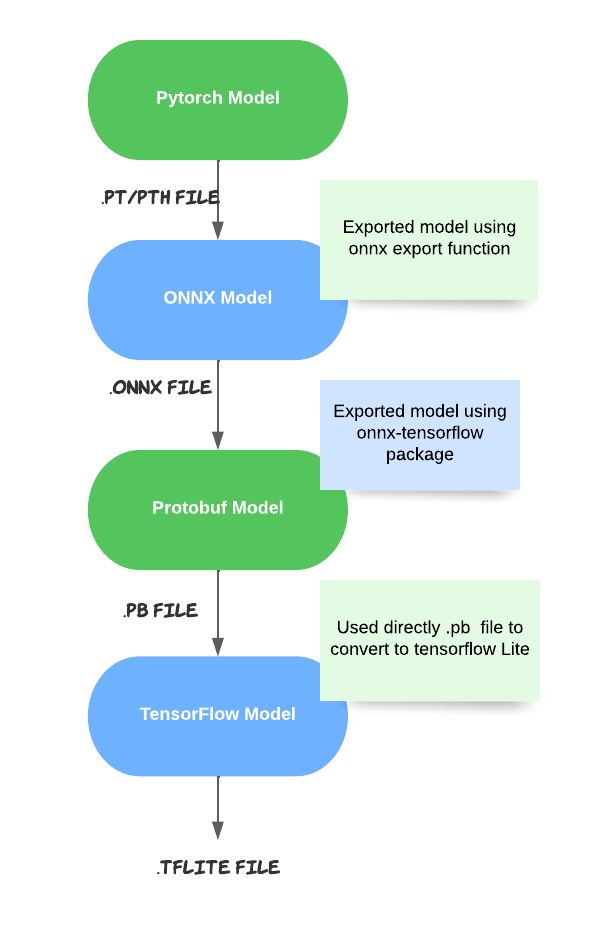
\includegraphics[scale=0.9]{img/model_conversion_process.png}
\caption{Model conversion process}
\label{fig:model_conversion_process}
\end{figure}


Following the above process or subset of the above process, I was able to convert our DNN ROS model[\ref{3model3}], team 2 model[\ref{3model5}] and team 20 [\ref{3model6}]. 


\chapter{ECG Arrhythmias classification} \label{chap5}

\section{Dataset employed} \label{5dataset}

PhysioNet presents an annual series of biomedical 'Challenges' that focus on unsolved clinical and basic science challenges in collaboration with the annual Computing in Cardiology (CinC) conferences. The National Institutes of Health (NIH), Google, MathWorks, and the Gordon and Betty Moore Foundation have all lent their support to these challenges. George Moody, of the Laboratory for Computational Physiology (LCP), directed these Challenges for the first 15 years (from 2000 to 2014), before retiring due to ill health. Gari Clifford of Emory University and the Georgia Institute of Technology has been leading the Challenges since 2015. In 2021, the ‘PhysioNet/Computing in Cardiology Challenges’ were renamed the ‘George B. Moody PhysioNet Challenges’ to honor George's lifetime contributions to the discipline, particularly his seminal work on the Challenges \cite{dataset1}.

The 2020 Challenge's purpose is to use 12-lead ECG records to detect clinical
diagnosis. Starting from the clinical data provided, the participants must implement an open-source algorithm that can automatically classify the
cardiac abnormality or abnormalities present in each 12-lead ECG recording
and provide a probability or confidence score for each of them, with an
emphasis on 27 diagnoses \ref{table:diagnoses_SNOMED} To determine the winner, the trained
models of the participants are run on hidden validation and test sets and
their performance is evaluated using a novel, expert-based evaluation
metric designed specifically for the 2020 Challenge. The team whose
algorithm achieves the highest score is the winner of the Challenge.

\begin{table}[H]
\begin{center}
\begin{tabular}{|c | c | c |}
 \hline
\textbf{Diagnosis} & \textbf{Code} & \textbf{Abbreviation} \\ [0.4ex] 
\hline \hline
1st degree AV block  & 270492004 & IAVB \\ \hline
Atrial fibrillation  & 164889003 & AF \\ \hline
Atrial flutter  & 164890007 & AFL \\ \hline
Bradycardia  & 426627000 & Brady \\ \hline
Complete right bundle branch block  & 713427006 & CRBBB \\ \hline
Incomplete right bundle branch block  & 713426002 & IRBBB \\ \hline
Left anterior fascicular block  & 445118002 & LAnFB \\ \hline
Left axis deviation  & 39732003 & LAD \\ \hline
Left bundle branch block  & 164909002 & LBBB \\ \hline
Low QRS voltages  & 251146004 & LQRSV \\ \hline
Nonspecific intraventricular conduction disorder  & 698252002 & NSIVCB \\ \hline
Pacing rhythm  & 10370003 & PR \\ \hline
Premature atrial contraction  & 284470004 & PAC \\ \hline
Premature ventricular contractions  & 427172004 & PVC \\ \hline
Prolonged PR interval  & 164947007 & LPR \\ \hline
Prolonged QT interval  & 111975006 & LQT \\ \hline
Q wave abnormal  & 164917005 & QAb \\ \hline
Right axis deviation  & 47665007 & RAD \\ \hline
Right bundle branch block  & 59118001 & RBBB \\ \hline
Sinus arrhythmia  & 427393009 & SA \\ \hline
Sinus bradycardia  & 426177001 & SB \\ \hline
Sinus rhythm  & 426783006 & NSR \\ \hline
Sinus tachycardia  & 427084000 & STach \\ \hline
Supraventricular premature beats  & 63593006 & SVPB \\ \hline
T wave abnormal  & 164934002 & Tab \\ \hline
T wave inversion  & 59931005 & TInv \\ \hline
Ventricular premature beats  & 17338001 & VPB \\ \hline

\hline\hline
\end{tabular}
\end{center}
\caption{Diagnoses, SNOMED CT codes and abbreviations for the 27 diagnoses that were scored for the Challenge.}
\label{table:diagnoses_SNOMED}
\end{table}

The data are from five different sources:
\begin{enumerate}
    \item CPSC Database and CPSC-Extra Database
    \item INCART Database
    \item PTB and PTB-XL Database
    \item The Georgia 12-lead ECG Challenge (G12EC) Database 
    \item Undisclosed Database
\end{enumerate}

The first source consists of three databases from the China Physiological Signal Challenge 2018 (CPSC2018), which took place in Nanjing, China at the 7th International Conference on Biomedical Engineering and Biotechnology \cite{dataset2}: the original public training dataset (CPSC), an unused dataset (CPSC-Extra), and the test dataset (the hidden CPSC set). The first two were shared as training sets, while the last one was split into validation and test set for the 2020 Challenge. This training set consists of two sets of 6,877 (male: 3,699; female: 3,178) and 3,453 (male: 1,843; female: 1,610) of 12-15 ECG recordings lasting from 6 seconds to 60 seconds. Each recording was sampled at 500 Hz.

The second source is the public dataset from the St. Petersburg Institute of Cardiological Technics (INCART) 12-lead Arrhythmia Database [15 V. Tihonenko, A. Khaustov, S. Ivanov, A. Rivin, and E. Yakushenko, “St Petersburg INCART 12-lead arrhythmia database”, PhysioBank, PhysioToolkit, and PhysioNet, 2008, doi: 10.13026/C2V88N.]. The dataset was shared as a training set. This database consists of 74 annotated recordings extracted from 32 Holter records. Each record is 30 minutes long and contains 12 standard leads, each sampled at 257 Hz.

The third source from the Physikalisch Technische Bundesanstalt (PTB) includes two public databases which were shared as training sets: the PTB Diagnostic ECG Database and the PTB-XL, a large publicly available electrocardiography dataset. The first PTB database contains 516 records (male: 377, female: 139). Each recording was sampled at 1000 Hz. The PTB-XL contains 21,837 clinical 12-lead ECGs (male: 11,379 and female: 10,458) of 10 second length with a sampling frequency of 500 Hz.


The fourth source is the Georgia 12-lead ECG Challenge (G12EC) Database. This is a new database, representing a large population from the Southeastern United States, and is split between the training, validation, and test sets. The validation and test set comprised the hidden G12EC set. This training set contains 10,344 12-lead ECGs (male: 5,551, female: 4,793) of 10 second length with a sampling frequency of 500 Hz.

The fifth source is a dataset from an undisclosed American institution that is geographically distinct from the other dataset sources. This dataset has never been posted publicly and contains 10,000 ECGs all retained as test data \cite{dataset2}. As the mentioned dataset was not disclosed, I didn't use that one in my experiments.

The actual count of all the diagnoses by each database can be found in Figure \ref{fig:diagnose_count_by_db}. That was obtained by taking the first arrtyhmia reported by each recording since each patient could contain more than one diagnose based on its ECG.

\begin{figure}[H]
\centering
\includegraphics[scale=0.3]{img/diagnose_count_by_db.png}
\caption{Number of recordings for each diagnosis by database}
\label{fig:diagnose_count_by_db}
\end{figure}

All data is provided in WFDB format. Each ECG recording has a binary \textbf{MATLAB v4 file} for the ECG signal data and a \textbf{text file} in WFDB header format describing the recording and patient attributes, including the diagnosis \cite{dataset3} \cite{dataset2} \cite{dataset4}.

\section{Centralized Learning} \label{5CL}

To get an understanding of the best performances achievable with the mentioned dataset I implemented a Centralized (or traditional) Learning. The latter means that I applied the analytical tools mentioned in \ref{chap4} over the complete dataset, without dividing it into clients. Then the main processes and results are summarized in the following literals.

\subsection{Data wrangling}

As mentioned in \ref{4dw}, the data wrangling process is usually the first step when dealing with a data-oriented problem. In this case, I placed the data in a Google Drive folder after downloading it from the official competition's website \cite{dataset3}. Afterwords, using Google Colaboratory I extracted and organized the information in Python. The representation of the ECG along the 12-leads can be examined in Figure \ref{fig:ecg_example_S0033}.

\begin{figure}[H]
\centering
\includegraphics[scale=0.35]{img/ecg_example_S0033.png}
\caption{12-lead ECG for recording S0033 of PTB database}
\label{fig:ecg_example_S0033}
\end{figure}

Then, the whole data (all the databases) and the features mentioned in \ref{4fe} were calculated. That process took almost 1 hour to run in an using the default configuration of Google Colab. Besides, for each recording I selected the first diagnose (arrhythmia) that appeared as the label to be predicted. The latter process ran in about 2 minutes.

\subsection{EDA}

Once the big dataset was loaded, it contained a total of 43,101 recordings and about 764 variables. From the latter, 650 features got created containing 14 competition provided features and 636 were spectral features. There were remaining 3 corresponded to the id of the recording, the database that it belongs to and the label (response variable to be predicted). Then, the first analysis need was to examine if the features contained any missing value. Using the function \texttt{bar} from the \texttt{missingno} library, I managed to explore the missing values. In figure \ref{fig:eda_missing} are depicted only the 50 first features' missing counts and percentage.

\begin{figure}[H]
\centering
\includegraphics[scale=0.32]{img/eda_missing.png}
\caption{Missing counts and percentage for 50 features of the complete dataset}
\label{fig:eda_missing}
\end{figure}

As shown in the previous chart, the missing percentage is considerably small (less than 0.1\%). For that reason, I decided to impute those missing values by using the mean (average) of each attribute. 

The second crucial aspect to investigate was the distribution of the response variable. Then, within the plot \ref{fig:label_ditro_alldata} it is shown the absolute count of each diagnose in the dataset.

\begin{figure}[H]
\centering
\includegraphics[scale=0.32]{img/label_ditro_alldata.png}
\caption{Label distribution for the complete dataset}
\label{fig:label_ditro_alldata}
\end{figure}

As evidenced in the previous chart, there are too many arrhythmias that don't have a big participation. That can lead to problems when trying to infer the predicted class of a recording, since there were not enough cases to learn the classifiers properly. That why those diagnoses with a participation smaller than 150 records where discarded from the analysis. With the previous filter, the selected data to work with got a size of 41,894 recordings distributed as shown in figure \ref{fig:diagnose_count_by_db_filtered}.

\begin{figure}[H]
\centering
\includegraphics[scale=0.32]{img/diagnose_count_by_db_filtered.png}
\caption{Number of recordings for each diagnosis by database for the filtered data}
\label{fig:diagnose_count_by_db_filtered}
\end{figure}

Besides, the final distribution of the labels ended up as shown in figure \ref{fig:label_ditro_filtered}. As expected, the most common diagnose was Normal Sinus Rhythm (NSR), which is the normal status for a ECG. In addition. the arrhythmia with one of the smallest participation turned out to be Sinus Arrhythmia (SA).

\begin{figure}[H]
\centering
\includegraphics[scale=0.32]{img/label_ditro_filtered.png}
\caption{Label distribution for the filtered dataset}
\label{fig:label_ditro_filtered}
\end{figure}

\subsection{Feature Selection and normalization}

In an analytical context, having a huge amount is a double-edged sword. On the one hand, the more information existing to predict a phenomena, the better. On the other hand, the computational time required to process to much information may lead to training times that are not affordable. Regarding the latter I decided to perform a feature selection step in order to determine the most important features to predict the arrhythmias. 

\begin{figure}[H]
\centering
\includegraphics[scale=0.23]{img/feature_importance.png}
\caption{Feature importance from XG-Boost algorithm (only the 50 best)}
\label{fig:feature_importance}
\end{figure}

The bar-plot in figure \ref{fig:feature_importance} depicted the most important features to predict the classes obtained by means of the XG-Boost method. The latter provides an automatic ranking of the most relevant features to classifier the ECGs. After having importance of features of all 650 features, next step was to try to reduce the unimportant features and
run the model. During various trial run and keeping F1-Score as primary metric reducing ranked features from 150 -100 F1-score went down from 0.56 to 0.52 and keeping it on 120 features it goes back to 0.56. So, in the end, 120 features got selected which leads to good enough accuracy and f1-
score compared to the one obtained using all the features.The best features turned out to be the Entropy for leads: 9, 11, 10; the percentile 5\% for lead 6; and the median for leads 1, 2.

As an additional tool to enhance the performance of the models there was an implementation of features \textbf{normalization}. In this case I tried three different techniques to transform the features to the same scale. The approaches tried were provided by the \texttt{sklearn} library in Python. Those are: \texttt{StandardScaler}, \texttt{MaxMinScaler} and \texttt{RobustScaler}. In the end, the scenario that provided the best results was using \texttt{RobustScaler}. 

\begin{equation} \label{robustscaler_eq}
X_{scale} = \frac{x_i - x_{med}}{x_{75} - x_{25}}
\end{equation}

\texttt{RobustScaler} [\ref{robustscaler_eq}] uses statistics that was resistant to outliers to scale features. The median removed, and the data scaled according to the quantile range (defaults to IQR: Interquartile Range). The interquartile range (IQR) is the distance between the first and third quartiles (25th and 3rd quantiles) (75th quantile). It is worth mentioning that centering and scaling happen independently on each feature by computing the relevant statistics on the samples in the given dataset.

\subsection{Balancing classes (arrhythmias)}

As depicted in \ref{fig:label_ditro_filtered}, the diagnoses have a imbalanced characteristic. The latter means that each category has a different participation over the data. That could represent a problem in the performance of the classifiers that will be proposed.

\begin{figure}[H]
\centering
\includegraphics[scale=0.4]{img/label_distro_ros.png}
\caption{Number of recordings for each diagnosis by database for the ROS oversampled data}
\label{fig:label_distro_ros}
\end{figure}

Then, two oversampling methods were proposed to deal with the imbalance issue. The first one is called \textbf{Random Oversampling (ROS)}. In the latter the minority classes are replicated together with its features. Besides, a down-sampling was applied to have a number of recording similar to the filtered dataset. In the end, the ROS dataset had 43,200 recordings. And as depicted in figure \ref{fig:label_distro_ros}, the distribution of the labels is much more similar among the arrhythmia categories.

\begin{figure}[H]
\centering
\includegraphics[scale=0.4]{img/label_distro_smote.png}
\caption{Number of recordings for each diagnosis by database for the SMOTE oversampled data}
\label{fig:label_distro_smote}
\end{figure}

The second oversampling technique used was SMOTE (SMT) \ref{3unbclass}. In the end, the SMOTE dataset had also 43,200 recordings. And as shown in figure \ref{fig:label_distro_smote}, the distribution of the labels is also similar among the arrhythmia categories.

\subsection{Fitted models and results}

With the previous pre-processing applied over the data, the following step was to adjust some Machine Learning models to the ECG's arrhythmias. During this step also other scenarios and considerations were employed \cite{datasplit}. A detailed explanation of the outlines is discussed in table \ref{table:scenarios_models}.

\begin{table}[H]
\begin{center}
\begin{tabular}{ ||p{3cm}||p{5cm}||p{4cm}|| }
 \hline
\textbf{Characteristic} & \textbf{Scenarios} & \textbf{Best approach}\\ [0.4ex] 
 \hline\hline
 Data Split & \%Train-\%Validation-\%Test: Option 1: 60\%-20\%-20\% Option 2: 70\%-10\%-10\% Option 3: 80\%-10\%-10\% Option 4: 90\%-5\%-5\% & Option 4: 90\%-5\%-5\%\\
\hline
Features normalization & Option 1: MinMaxScaler \hspace{10 mm} Option 2: StandardScaler \hspace{10 mm} Option 3: RobustScaler & Option 3: RobustScaler \\
\hline
Sampling rate & Option 1: 257Hz \hspace{10 mm} Option 2: 500Hz & Option 1: 257Hz \\
\hline
Features employed & Option 1: Baseline features Option 2: Baseline features + Spectral features & Option 2: Baseline features + Spectral features \\
\hline\hline
\end{tabular}
\end{center}
\caption{Scenarios tried during modelling phase}
\label{table:scenarios_models}
\end{table}

In the previous table are depicted the best approaches that managed to get the best performances (in terms of Accuracy, Recall, Precision, F1-Score and Overall Score). Moreover, in figure \ref{fig:cl_oindex_methods} is shown the detailed behaviour of each one of the algorithms employed.

\begin{figure}[H]
\centering
\includegraphics[scale=0.5]{img/cl_oindex_methods.png}
\caption{Overall Index for methods employed in Centralized Learning (CL)}
\label{fig:cl_oindex_methods}
\end{figure}

Within the previous results it is easy to realize that the champion model is the one that applies Catboost over the ROS data. The latter obtained an overall index close to 0.68. Competition team which ranked 2 is at the second position having overall index as 0.64. This model was trained over above \ref{table:scenarios_models} scenario having trained data as 90\%, 5\% validation data and 5\% for testing and same pattern has been followed on team 20 analysis. Nevertheless, the Deep Neural Network (DNN) applied over the ROS data has a close behaviour, having a the mentioned metric in 0.61. Finally, LSTM and XG-Boost does not perform that well compared to the other models. An additional point to mention is that both Catboost and DNN used over the ROS dataset does not show any sign of overfitting since the metrics for train, validation and test sets are almost the same. As for team 2 and team 20 in the above figure train and validation overall index is not shown because they followed their own pattern keeping in mind the competition score during training and validation. 

\begin{figure}[H]
\centering
\includegraphics[scale=0.55]{img/cl_accuracy_methods.png}
\caption{Accuracy for methods employed in Centralized Learning (CL)}
\label{fig:cl_accuracy_methods}
\end{figure}

\begin{figure}[H]
\centering
\includegraphics[scale=0.55]{img/cl_f1score_methods.png}
\caption{F1-Score for methods employed in Centralized Learning (CL)}
\label{fig:cl_f1score_methods}
\end{figure}

A similar analysis can be derived from figures \ref{fig:cl_accuracy_methods} and \ref{fig:cl_f1score_methods}, where the Accuracy and F1-Score are shown. In terms of Accuracy, Catboost got 0.67, team 2 got 0.64 and DNN got 0.61 while applied over the ROS dataset. It is important to clarify that using Accuracy is not a the best metrics in this dataset since the labels are heavily unbalanced. For that reason, it is better to use the F1-Score. which is more robust to the imbalanced datasets. Then, in terms of F1-Score, Catboost obtained a 0.67, team 2 model got 0.63 and DNN 0.62.

\begin{figure}[H]
\centering
\includegraphics[scale=0.6]{img/time_cl_teams.png}
\caption{Execution times for the methods used in CL}
\label{fig:times_cl}
\end{figure}

Finally, a measurement of the time taken to train for each model was included. As shown in figure \ref{fig:times_cl}, Team 20 model took almost 619 minutes, team 2 took 156 minutes and Catboost took almost 35 minutes to run. On the other hand, DNN and LSTM are algorithms that employed a few time in training (close to 4 minutes in average). Finally, Catboost is the slowest method, although it generates the best results. In counter position, DNN is the fastest method, and the performance is NOT quite different from Catboost and team 2 model. Team 2 and team 20 models took this much time because they are end to end models instead of feature based model. Although I have done some experiments on team 2 which will be explained below. 


\section{Conversion to Tensorflow Lite } \label{5CTL}

 We can convert potentially any model that is built using TensorFlow core libraries and tools. Once you've built a model with TensorFlow core, you can convert it to a smaller, more efficient ML model format called a TensorFlow Lite. Also, there are other advanced steps related to it if your model is built using tensorflow core libraries by looking at the steps here  \ref{fig:model_conversion_process} we can convert models that are built using either in Pytorch or Matlab. 
 
 
\subsection{Model 1(XGBoost) and Model 2(Catboost) conversion}\label{5CTLM1M2}

As both of \href{https://xgboost.readthedocs.io}{XGBoost} and \href{https://catboost.ai}{Catboost} are not built using Tensorflow even there is no direct conversion available I opted out to use trained models built on top of CatBoost and XGBoost. Just to keep in mind that both of these libraries somehow support directly or indirectly iOS platform but not the android. As after conversion I am going to use directly in both iOS/Android to see how they perform in real world scenarios. 

\subsection{Model 3(LSTM)}\label{5CTLM3}

LSTM model is built on top of Tensorflow so it was convertable to tensorflow lite. If we look at LSTM models of simple LSTM, LSTM ROS, LSTM SMOTE, better F1-score and overall index is achieved by simple LSTM model with 0.49 overall index and 0.47 F1-score. LSTM had one problem during conversion step it had two sub graphs which is not supported by tensorflow lite models. To overcome this problem \textbf{TFLite LSTM op } was used and at the end we get the graph that had only one subgraph.


\begin{figure}[H]
\centering
\includegraphics[scale=0.7]{img/lstm_conversion_comparison.png}
\caption{Tensorflow LSTM model's graph to Tensorflow Lite model's graph comparison}
\label{fig:lstm_conversion_comparison}
\end{figure}


As you can see in \ref{fig:lstm_conversion_comparison}, LSTM Tensorflow original model and Tensorlow Lite model after conversion step taken place using TFLite LSTM op. 

\subsection{Model 4(DNN)}\label{5CTLM4}

As DNN model was also built using Tensorflow with 4 fully connected layers 3 with 500 neurons output in each and relu as activation function with output. In the fourth layer, it has to output 27 classes of arythmia's with probabilities so it using Softmax in the last layer. To look at its graph in tensorflow lite model it is not that interesting and the only intresting thing to note that tensorflow lite as I have converted only support one input at a time and Tensorflow one can support batches of inputs as well. As, I have to use Tensoflow lite version in mobile so most probably it will be given an input to classify one at a time. 


\begin{figure}[H]
\centering
\includegraphics[scale=0.7]{img/dnn_conversion_comparison.png}
\caption{Tensorflow DNN model's graph to Tensorflow Lite model's graph comparison}
\label{dnn_conversion_comparison}
\end{figure}


\subsection{Model 5 - Challenge Team 2}\label{5CTLM5}

As challenge 2 team was using Pytorch instead of Tensorflow as primary framework library to build the model. I have to convert the model following all the steps mentioned in \ref{fig:model_conversion_process}. So, first trained model .pt file is converted to ONNX format and get tested, then it got converted to .pb file and at the end when .pb get imported to tensorflow it got directly converted to Tensorflow lite. As challenge team 2 was using ensemble approach where they were using 5 models which got trained over shuffled dataset for training and validation. We will look at the first model in .pt format how it looks and then converted model in Tensorflow Lite as comaprison. Also, this model length is too big to compare it here I will be using first few layers as comparison here. 

\begin{figure}[H]
\centering
\includegraphics[scale=0.7]{img/resnetse_conversion_comparison.png}
\caption{Pytorch ResnetSE 18 model's graph to Tensorflow Lite model's graph comparison }
\label{resenet18_conversion_comparison}
\end{figure}

As we can see in \ref{resenet18_conversion_comparison} during conversion to tensorflow lite there are too many operation that gets performed including pad, Transpose, Reshape, Mul and etc. So, we can conclude that in conversion process to Tensorflow Lite there are additional operations gets added to model graphs to support some of complex operations. 


\subsection{Model 6 - Challenge Team 20}\label{5CTLM6}

As Challenge team 20, worked directly on Tensorflow framework library it was easy to convert the model to Tensorflow Lite directly. Lets look at the original model and converted model comparison side by side. It is also important to mentioned that as they were training 10 different models using shuffled dataset and I choose the one for comaprison which were performing better in Accuracy, F1 measure and overall index. It is important to note that difference between these models was really small it terms of metrics as mentioned before. Model graph length is too big to paste it here so I will be comparing first few layers of it as in the case of Model 5. \ref{5CTLM5} 


\begin{figure}[H]
\centering
\includegraphics[scale=0.7]{img/team20_conversion_comparison.png}
\caption{Tensorflow Team 20 model's graph to Tensorflow Lite model's graph comparison}
\label{team20_conversion_comparison}
\end{figure}

Looking at above figure \ref{team20_conversion_comparison}, we can clearly see that in tensorflow lite graph there are multiple other operations that we haven't seen befofe like Sub, SquaredDifference, Mean, Rsqrt etc. It is evident all the complex operations get converted to more simpler operations in tensorflow lite format of the model.  



\subsection{Metrics of models}

As written previously, Catboost and XGBoost \ref{5CTLM1M2} are not convertible directly to tensorflow lite. Besides that other models were convertible and it was only worth to look at the models that performed well in terms of accuracy, f1-score and overall index because they will be later used for detecting arythmias in mobile applications. So, DNN ROS with overeall index as 0.62, LSTM with overall index as 0.49, Team 2 model with overall index as 0.64 and Team 20 model(CNN+Rule Based) with overall index of 0.47 was chosen for below analysis. 


\begin{figure}[H]
\subfloat[DNN ROS]{\includegraphics[width = 3in]{img/dnnros_metrics.png}} 
\subfloat[LSTM]{\includegraphics[width = 3in]{img/lstm_metrics.png}}\\
\subfloat[Team 2]{\includegraphics[width = 3in]{img/team2_metrics.png}}
\subfloat[Team 20]{\includegraphics[width = 3in]{img/team20_metrics.png}} 
\caption{Metrics of models comparing side by side with original model and TF Lite version of the model}
\label{metricsafterconversion}
\end{figure}

If we look at above figures we can clearly see that a little drop in every metric after the model is converted to tensorflow lite. As, I didn't wanted the models to be quantize more so that their accuracy, f1-score decreases so I opted for tensorflow lite default conversion operations. 


Now if we move toward looking at how much time it takes the to get output from the model either before converting and after converting. There is huge difference when model is converted and we wanted to get the output from the model. It takes slighly and in case of hafty model it takes a lot more time. In real world scenario as we will not be using batching, or multiple inputs to get the output from the model because of that all above converted models only accept one input at a time. 

\begin{figure}[H]
\centering
\includegraphics[scale=0.45]{img/inference_time_of_converted_models.png}
\caption{Inference Time in minutes of original and converted models}
\label{inference_time_of_converted_models}
\end{figure}

If we look at above \ref{figure:inference_time_of_converted_models} figure we can clearly see that LSTM and DNN ROS models are way faster than Team 2 and Team 2. LSTM and DNN ROS models even after conversion is taking less than 0.30 sec to execute. To put it more precisely orginal DNN on test dataset with 2095 features takes 19 seconds to get outputs and .13 seconds for inference in case of converted model which is even less than original model. If we look at LSTM it does the same 13 seconds for original model and 067 seconds on converted model. This means that somehow both DNN and LSTM has to perform less operations and gets lighter and efficient after conversion. While on the other hand Team 2 and Team 20 models takes significantly too much time to output the results. More precisely, in case of Team 2 model it takes 1826 seconds to output 2095 results and 66960 seconds in case of converted model which raises concerns because its significantly slower than original model. As in the case of team 20 inference on original model was significantly smaller as 9.4 seconds and inference on converted model was huge slower 80232 seconds. It maybe due to CPU or GPU inference, I didn't get a chance to look at it. 

\begin{table}
\centering
\begin{tabular}{ |p{5cm}||p{3cm}|p{3cm}|}
 \hline
 \multicolumn{3}{|c|}{Size of Models} \\
 \hline
 Model's Name& Original Size&Converted size\\
 \hline
 DNN ROS   & 2.2MB   &   569KB\\
 LSTM&  82KB   & \textbf{29KB} \\
 TEAM\#2 &33.8MB & 9.6MB\\
 TEAM\#20  & 138.8MB & 11.6MB\\
 \hline
\end{tabular}
 \caption{\label{tab:models_size_after_conversion}Comparison of model size from original to converted models}
 \end{table}
 
 As you can see from \ref{tab:models_size_after_conversion}, the smallest model is LSTM and it even gets smaller when converted to tensorflow lite. Team \#20 model is really huge and its get converted to 11.6MB. Maybe because of that it takes time during inference. 
 
\subsection{Models Deployment}

As part of the models testing on mobile devices after conversion. LSTM, DNN ROS and Team \#2 model has been deployed on the mobile devices while building a small demo application using flutter. \href{https://flutter.dev/}{Flutter} is an open-source UI software development kit created by Google. As flutter supports Tensorflow Lite models only Catboost, XGBoost are not deployed, as well as Team \#20 model because accuracy,f1-score of the team \#20 model is very less. 

In the demo application, two main packages has been used \href{https://pub.dev/packages/tflite\_flutter}{tflite\_flutter} and \href{https://pub.dev/packages/csv}{csv}. \textit{csv} package has been used to read csv files and \textit{tflite\_flutter} is used to inference converted models. 

\textbf{DNN ROS and LSTM}

For DNN ROS and LSTM, I saved the features of test dataset 5\% after normalizing and standardizing as explained above in csv file. This csv file is used directly for inputs to the models. Then as both models are trained to classify single arythmia. Output of the model is based on classifying 27 arythmia's so whichever arythmia type is at highest probability is shown as predicted and then two more types according to highest probabilities is shown in \ref{dnn_deloyment} 


\begin{figure}[H]
\centering
\includegraphics[scale=0.4]{img/dnn_deloyment.png}
\caption{iOS and Android DNN model classification example}
\label{dnn_deloyment}
\end{figure}

\begin{figure}[H]
\centering
\includegraphics[scale=0.4]{img/lstm_deployment.png}
\caption{iOS and Android LSTM model classification example}
\label{dnn_deloyment}
\end{figure}

\textbf{Competence Team \# 2}

For competence team \# 2, as they were using end to end model to classify 12-lead ECG, so for each input after pre processing was saved as one csv file instead .mat file in original dataset and age, sex and dx is saved separately as well in other csv file to provide it to the model. As competence team \# 2 was using ensemble model, combining 5 of them to output the results for final classification there has been post processing done on mobile application as it was in original source code provided by \ref{fig:team_two_network_2}. If we look at closely their model is doing multi class classification instead of predicting one arrhythmia at time because a patient can have more than one arrhythmia. Also, during prediction probabilities are divided into for how many arrhythmias its predict. For example if the model is predicting two different arrhythmia's based on 12-lead ECG it will make whole percentage as 200\% instead of 100\%. 

\begin{figure}[H]
\centering
\includegraphics[scale=0.4]{img/lstm_deployment.png}
\caption{iOS and Android Team \# 2 model classification example}
\label{dnn_deloyment}
\end{figure}




\section{Federated Learning} \label{5FL}

Leveraged on the Centralized Learning method mentioned, it is time to immerse in the Federated Learning (FL) approach executed for this ECG dataset. With the CL it was possible to get an overall performance with the best technique and scenarios to be applied. To deal with the FL proposed IID approach has been choose for analysis. 

\subsection{IID approach}

This approach was based on the idea of using the whole dataset containing 41,894 registers and divide it in 4 different datasets (local nodes). As a parenthesis, the decision of the number of local nodes was based on selecting at least 30 diagnoses for the rarest arrhythmia. Due to the stratified random splitting, the mentioned data in each local node (or client) will be Independent and Identically Distributed (IID) \ref{proposed_approaches}. This scenario is not completely realistic since usually the ECGs shared in multiple devices are Non-IID. Nevertheless, it is worth to try and see how the FL approach will perform over the data.

\begin{figure}[H]
\centering
\includegraphics[scale=0.4]{img/fl_label_distro_filtered.png}
\caption{Label distribution for the filtered dataset by each local node}
\label{fig:fl_label_distro_filtered}
\end{figure}

As depicted in figure \ref{fig:fl_label_distro_filtered}, the distribution among the 4 local nodes seems IID. The later means that the diagnoses along the devices will be the same. Besides, each local node contains 9,426 recordings. The same occurs for the ROS and SMOTE datasets when dividing them in 4 clients, as is shown inf figures \ref{fig:fl_label_distro_filtered_ROS_SMT}. Of course, in this case all the diagnoses have almost the same participation across the nodes, making them IID and balanced.

\begin{figure}[H]
\centering
\includegraphics[scale=0.4]{img/fl_label_distro_filtered_ROS_SMT.png}
\caption{Label distribution for the ROS and SMOTE datasets by each local node}
\label{fig:fl_label_distro_filtered_ROS_SMT}
\end{figure}

Once the four datasets were settled, the modelling part can be performed. As a reminder, in the FL technique, each local node will train a model and later it will send the weights to a global node where the weights are averaged and updated back in each client. Then, the DNN and LSTM methodologies were used to classify the ECG's arrhythmias. It is relevant to highlight that Catboost and XG-Boost were not employed in this step. The former was discarded for its low performance and the latter due to its huge training time. Moreover, it the consulted bibliography, it is not common to use those ML techniques within the FL.

\begin{figure}[H]
\centering
\includegraphics[scale=0.6]{img/fl_iid_methods.png}
\caption{Overall Index for methods employed in Federated Learning (FL)}
\label{fig:fl_iid_methods}
\end{figure}

As depicted in figure \ref{fig:fl_iid_methods}, the best results where obtained using the DNN with the ROS datasets. The later got an overall index of 0.55 in the test set. On the other hand, the best performance for LSTM was obtained with the original data, although it is worst than the DNN ROS model. The latter means that applying oversampling techniques doesn't improve the result of the models in the LSTM approach. But, when using ROS, the performance of the FL model is the most useful compared to all the techniques.

\begin{figure}[H]
\centering
\includegraphics[scale=0.6]{img/times_fl_iid.png}
\caption{Execution times for the methods used in FL IID approach}
\label{fig:times_fl_iid}
\end{figure}

Analyzing figure \ref{fig:times_fl_iid} it is possible to get that the oversampling techniques cause the running time to increase \cite{fl28}. In detail, the slowest approach ended up being the DNN ROS with 17 minutes. Comparing the results to the CL approach, the DNN method with FL runs faster with similar results. On the other hand, DNN ROS and SMOTE ran slower and with a slower performance than the CL. Finally, LSTM, in general, has a lower performance than DNN, but runs faster.

With FL it is possible to control the performance that the models has in each local node. The latter is relevant to understand if there is some node that is under-performing, compared to the others.

\begin{figure}[H]
\centering
\includegraphics[scale=0.4]{img/iid_local_nodes_acc.png}
\caption{Train and Validation accuracy among local nodes for DNN ROS}
\label{fig:iid_local_nodes_acc}
\end{figure}

In figure \ref{fig:iid_local_nodes_acc} is depicted the behaviour of each local node with respect to the accuracy for both the training and validation datasets. In general, the models among the clients have a similar behaviour. All of them get stabilized around the 5th epoch. It is important to clarify that the accuracy for train and validation seems considerably far from each other. The latter would mean that the models are over-fitting. Nevertheless, the train sample is an over-sampled data while the validation is a part of the original data, then, it is expected to such a behaviour.

In a a FL environment there is a concept called \textbf{communication round} (comm round). The latter begins when a model is trained inside each one of the local nodes. Later the weights of the models are passed to the global node to be aggregated there. And finally, the communication round finishes when each local model is updated with the new weights. Then, it is expected that in each comm round the performance of the model increases. Moreover, it should get stable after some trials.

\begin{figure}[H]
\centering
\includegraphics[scale=0.4]{img/comm_round_metrics_DNNROS.png}
\caption{Metrics along communication rounds for DNN ROS (the best model)}
\label{fig:comm_round_metrics_DNNROS}
\end{figure}

Figure \ref{fig:comm_round_metrics_DNNROS} establishes the behaviour of each metrics along the communication rounds. As expected, the performances gets stable after the 15th comm round approximately. It is relevant to notice that in the first comm round the Precision starts high and the Recall low. But after some updates both measures get steady. Moreover, the curves for train, validation and test are close. The latter means that there are not signals of over fitting.


\begin{table*}[ht]
\begin{center}
% \begin{tabular}{ ||p{1cm}||p{1cm}||p{1cm}||p{1cm}||p{1cm}||p{1cm}||}
% \resizebox{\width}{!}{
\begin{adjustbox}{width=\textwidth}
\begin{tabular}{|l|*{5}{c}|*{5}{c}|}

\cline{1-11} & \multicolumn{5}{c|}{CL} & \multicolumn{5}{c|}{FL IID}       \\  \cline{2-11}
 Method & \multicolumn{1}{c|}{Accuracy} & \multicolumn{1}{c|}{Precision}& \multicolumn{1}{c|}{Recall}& \multicolumn{1}{c|}{F1-Score} & \multicolumn{1}{c|}{Time} & \multicolumn{1}{c|}{Accuracy} & \multicolumn{1}{c|}{Precision}& \multicolumn{1}{c|}{Recall}& \multicolumn{1}{c|}{F1-Score} & \multicolumn{1}{c|}{Time} \\ 
 \hline \hline
\multicolumn{1}{|l|}{Competence Team \#2 \cite{second_team}} & 0.645 & 0.640 & 0.645& 0.631 & 155 & - & - & - & - & - \\

\multicolumn{1}{|l|}{Competence Team \#20 \cite{team_20}} & 0.472 & 0.515 & 0.472 & 0.440 & 618 & - & - & - & - & - \\
\multicolumn{1}{|l|}{Inspirational DNN \ref{3model4}} & 0.50 & 0.46 & 0.50 & 0.47 & \textbf{1.4} & - & - & - & - & -  \\
\multicolumn{1}{|l|}{Inspirational LSTM \ref{3model3}} & 0.50 & 0.45 & 0.50 & 0.46 & 2.1 & - & - & - & - & -  \\
\hline\hline
\multicolumn{1}{|l|}{XG-BOOST} & 0.52 & 0.49 & 0.52 & 0.49 & 9.4 & - & - & - & - & -  \\
\multicolumn{1}{|l|}{XG-BOOST ROS} & 0.45 & 0.58 & 0.45 & 0.47 & 15.7 & - & - & - & - & - \\ 
\multicolumn{1}{|l|}{XG-BOOST SMOTE} & 0.48 & 0.55 & 0.48 & 0.49 & 15.4 & - & - & - & - & -  \\
\multicolumn{1}{|l|}{CATBOOST} & 0.55 & 0.54 & 0.55 & 0.53 & 34.5 & - & - & - & - & - \\
\multicolumn{1}{|l|}{CATBOOST ROS} & \textbf{0.67} & \textbf{0.72} &\textbf{ 0.67 }& \textbf{0.67} & 36.4 & - & - & - & - & -  \\
\multicolumn{1}{|l|}{CATBOOST SMOTE} & 0.64 & 0.66 & 0.64 & 0.64 & 35.5 & - & - & - & - & -  \\
\hline\hline
\multicolumn{1}{|l|}{DNN} & 0.50 & 0.47 & 0.50 & 0.47 & 2.8 & 0.46 & 0.53 & 0.45 & 0.49 & 2.3  \\
\multicolumn{1}{|l|}{DNN ROS} & 0.61 & 0.66 & 0.61 & 0.61 & 3.8 & \textbf{0.55} & \textbf{0.59} & \textbf{0.54} & \textbf{0.55} & 16.3  \\
\multicolumn{1}{|l|}{DNN SMOTE} & 0.60 & 0.64 & 0.60 & 0.60 & 4.3 & 0.52 & 0.58 & 0.52 & 0.51 & 16.8  \\
\hline\hline
\multicolumn{1}{|l|}{LSTM} & 0.51 & 0.47 & 0.51 & 0.39 & 4.3 & 0.48 & 0.58 & 0.48 & 0.52 & \textbf{1.0}  \\ 
\multicolumn{1}{|l|}{LSTM ROS} & 0.38 & 0.51 & 0.38 & 0.39 & 4.9 & 0.39 & 0.48 & 0.38 & 0.38 & 4.7  \\
\multicolumn{1}{|l|}{LSTM SMOTE} & 0.39 & 0.49 & 0.39 & 0.39 & 2.7 & 0.39 & 0.47 & 0.39 & 0.38 & 5.3  \\
\hline
\end{tabular}
% }
\end{adjustbox}
\end{center}
\caption{Metrics for Centralized (CL) and IID Federated Learning (FL -IID) in the test data set. Also included execution time for training in minutes.}
\label{table:metrics_CL_FLIID}
\end{table*}

The table \ref{table:metrics_CL_FLIID} includes a summary of all the techniques implemented with the data in the IID and Centralized (CL) approaches. It is remarkable to mention that Catboost ROS outperform Competence Team \# 2 model. DNN ROS is model that have good enough accuracy and f1-score which can be easily deployed to any small memory devices after conversion.  

\chapter{Conclusions} \label{chap6}

\section{Summary} \label{6summary}
xx


\section{Future Developments} \label{6futuredevelopments}

xx



\backmatter
% bibliography
\cleardoublepage
\phantomsection
\bibliographystyle{unsrt} % BibTeX style
\bibliography{bibliography} % BibTeX database without .bib extension

\end{document}
